\documentclass[cs4size,a4paper,10pt]{ctexart}   

\linespread{1.5}
\usepackage{geometry}%用于设置上下左右页边距
	\geometry{left=2.5cm,right=2.5cm,top=3.2cm,bottom=2.7cm}
\usepackage{xeCJK,amsmath,paralist,enumerate,booktabs,multirow,graphicx,subfig,setspace,listings,lastpage,hyperref}
\usepackage{amsthm, amssymb, bm, color, framed, graphicx, hyperref, mathrsfs}
\usepackage{mathrsfs}  
	\setlength{\parindent}{2em}
	\lstset{language=Matlab}%
\usepackage{fancyhdr}
\usepackage{graphicx}
\usepackage{subfloat}
\usepackage{listings}
\usepackage{xcolor}
\usepackage{float}
\usepackage{paralist}
\usepackage{setspace}
\usepackage{titlesec}
\usepackage{enumitem}
\usepackage{hyperref}
\usepackage{multirow}
\usepackage{threeparttable}
\usepackage{multicol}



\hypersetup{
	colorlinks=true,
	linkcolor=black
}

\setenumerate{partopsep=0pt,topsep=0pt}
\setitemize{itemsep=0pt,partopsep=0pt,topsep=0pt}

\titlespacing*{\section}{0pt}{3pt}{3pt}
\titlespacing*{\subsection}{0pt}{2pt}{2pt}
\titlespacing*{\subsubsection}{0pt}{1pt}{1pt}
\titlespacing*{\paragraph}{0pt}{0pt}{0pt}

\ctexset{secnumdepth=4,tocdepth=4}
\setlength{\parindent}{0pt}
\setstretch{1.2}


\setCJKmainfont[BoldFont={FZHei-B01},ItalicFont={FZKai-Z03}]{FZShuSong-Z01} 
\setCJKsansfont[BoldFont={FZHei-B01}]{FZKai-Z03} 
\setCJKmonofont[BoldFont={FZHei-B01}]{FZFangSong-Z02}
\setCJKfamilyfont{zhsong}{FZShuSong-Z01} 
\setCJKfamilyfont{zhhei}{FZHei-B01} 
\setCJKfamilyfont{zhkai}[BoldFont={FZHei-B01}]{FZKai-Z03} 
\setCJKfamilyfont{zhfs}[BoldFont={FZHei-B01}]{FZFangSong-Z02} 
\renewcommand*{\songti}{\CJKfamily{zhsong}} 
\renewcommand*{\heiti}{\CJKfamily{zhhei}} 
\renewcommand*{\kaishu}{\CJKfamily{zhkai}} 
\renewcommand*{\fangsong}{\CJKfamily{zhfs}}


\definecolor{mKeyword}{RGB}{0,0,255}          % bule
\definecolor{mString}{RGB}{160,32,240}        % purple
\definecolor{mComment}{RGB}{34,139,34}        % green
\definecolor{mNumber}{RGB}{128,128,128} 

\lstdefinestyle {njulisting} {
	basewidth = 0.5 em,
	lineskip = 3 pt,
	basicstyle = \small\ttfamily,
	% keywordstyle = \bfseries,
	commentstyle = \itshape\color{gray}, 
	basicstyle=\small\ttfamily,
	keywordstyle={\color{mKeyword}},     % sets color for keywords
	stringstyle={\color{mString}},       % sets color for strings
	commentstyle={\color{mComment}},     % sets color for comments
	numberstyle=\tiny\color{mNumber},
	numbers = left,
	captionpos = t,
	breaklines = true,
	xleftmargin = 2 em,
	xrightmargin = 2 em,
	frame=tlrb,
	tabsize=4
}

\lstset{
style = njulisting, % 调用上述样式 
flexiblecolumns % 允许调整字符宽度
}


%================= 基本格式预置 ===========================
\usepackage{fancyhdr}
\pagestyle{fancy}
\lhead{\textsc{Computer Networking}}
\rhead{第一章\ 计算机网络概述}
\cfoot{\thepage}
\renewcommand{\headrulewidth}{0.4pt}
\renewcommand{\theenumi}{(\arabic{enumi})}
\CTEXsetup[format={\bfseries\zihao{-3}}]{section}
\CTEXsetup[format={\bfseries\zihao{4}}]{subsection}
\CTEXsetup[format={\bfseries\zihao{-4}}]{subsubsection}


\renewcommand{\contentsname}{目录}  
\begin{document}

	\begin{center}
		{\huge\textbf{第一章\ 计算机网络概述}}
	\end{center}
	%---------目录---------% 
	\pagenumbering{Roman}
	\tableofcontents
	\clearpage

 	%---------正文---------% 
	\pagenumbering{arabic}
	\setcounter{page}{1}
	\setlength{\parskip}{0.65em}
	
	\section{计算机网络在信息时代的作用}
	\begin{itemize}
		\item 计算机网络已由一种通信基础设施发展成为一种重要的信息服务基础设施
		\item 计算机网络已经像水、电、煤气这些基础设施一样,成为我们生活中不可或缺的一部分
	\end{itemize}

	\section{互联网概述}

	\subsection{网络的网络}
	\begin{itemize}
		\item 计算机网络(简称为网络)由若干结点(node)和连接这些结点的链路(link)组成
		\item 网络中的结点可以是计算机、集线器、交换机或路由器等
		\item 网络之间还可以通过路由器互连起来,这就构成了一个覆盖范围更大的计算机网络,这样的网络称为互连网
		\item 互连网是“网络的网络”(network of networks)
		\item - 网络把许多计算机连接在一起,而互连网则把许多网络通过路由器连接在一起。与网络相连的计算机常称为主机
		\item 网络互连并不是把计算机仅仅简单地在物理上连接起来,还必须在计算机上安装许多使计算机能够交换信息的软件才行
	\end{itemize}

	\begin{figure}[H]
		\centering
		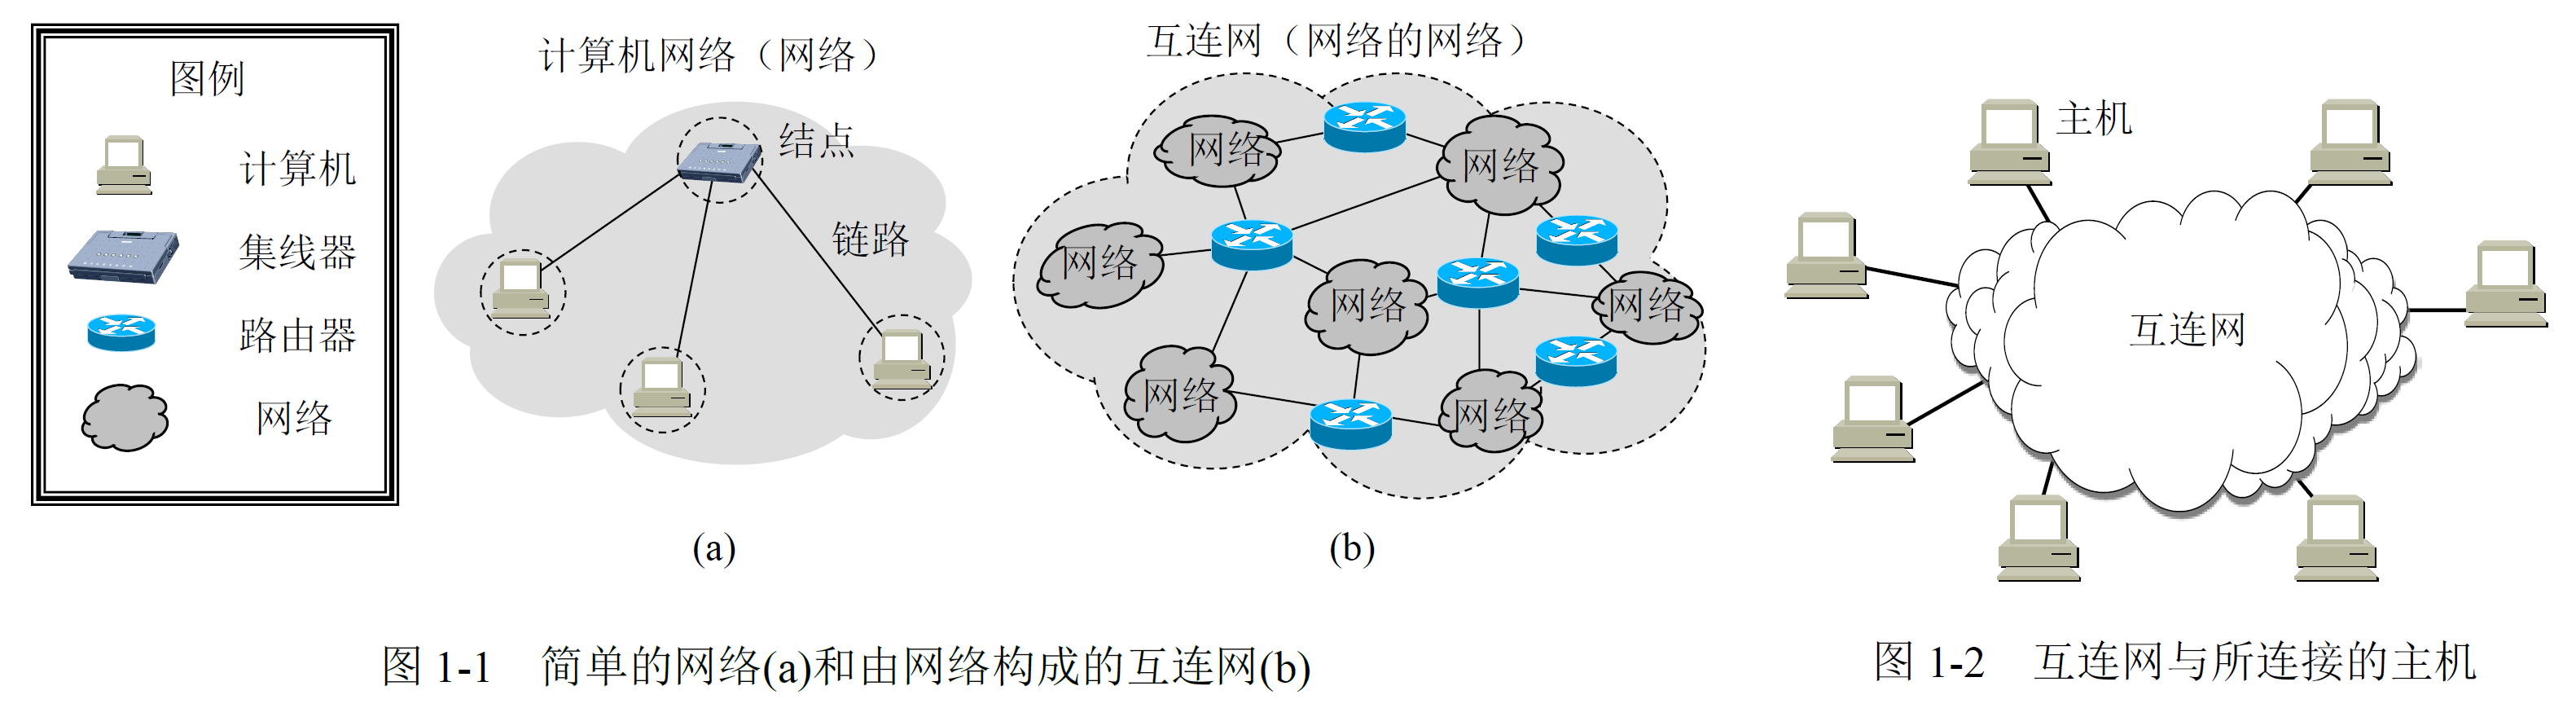
\includegraphics[width=0.9\textwidth]{img/1.1}
	\end{figure}

	\subsection{互联网基础结构发展的三个阶段}
	\begin{figure}[H]
		\centering
		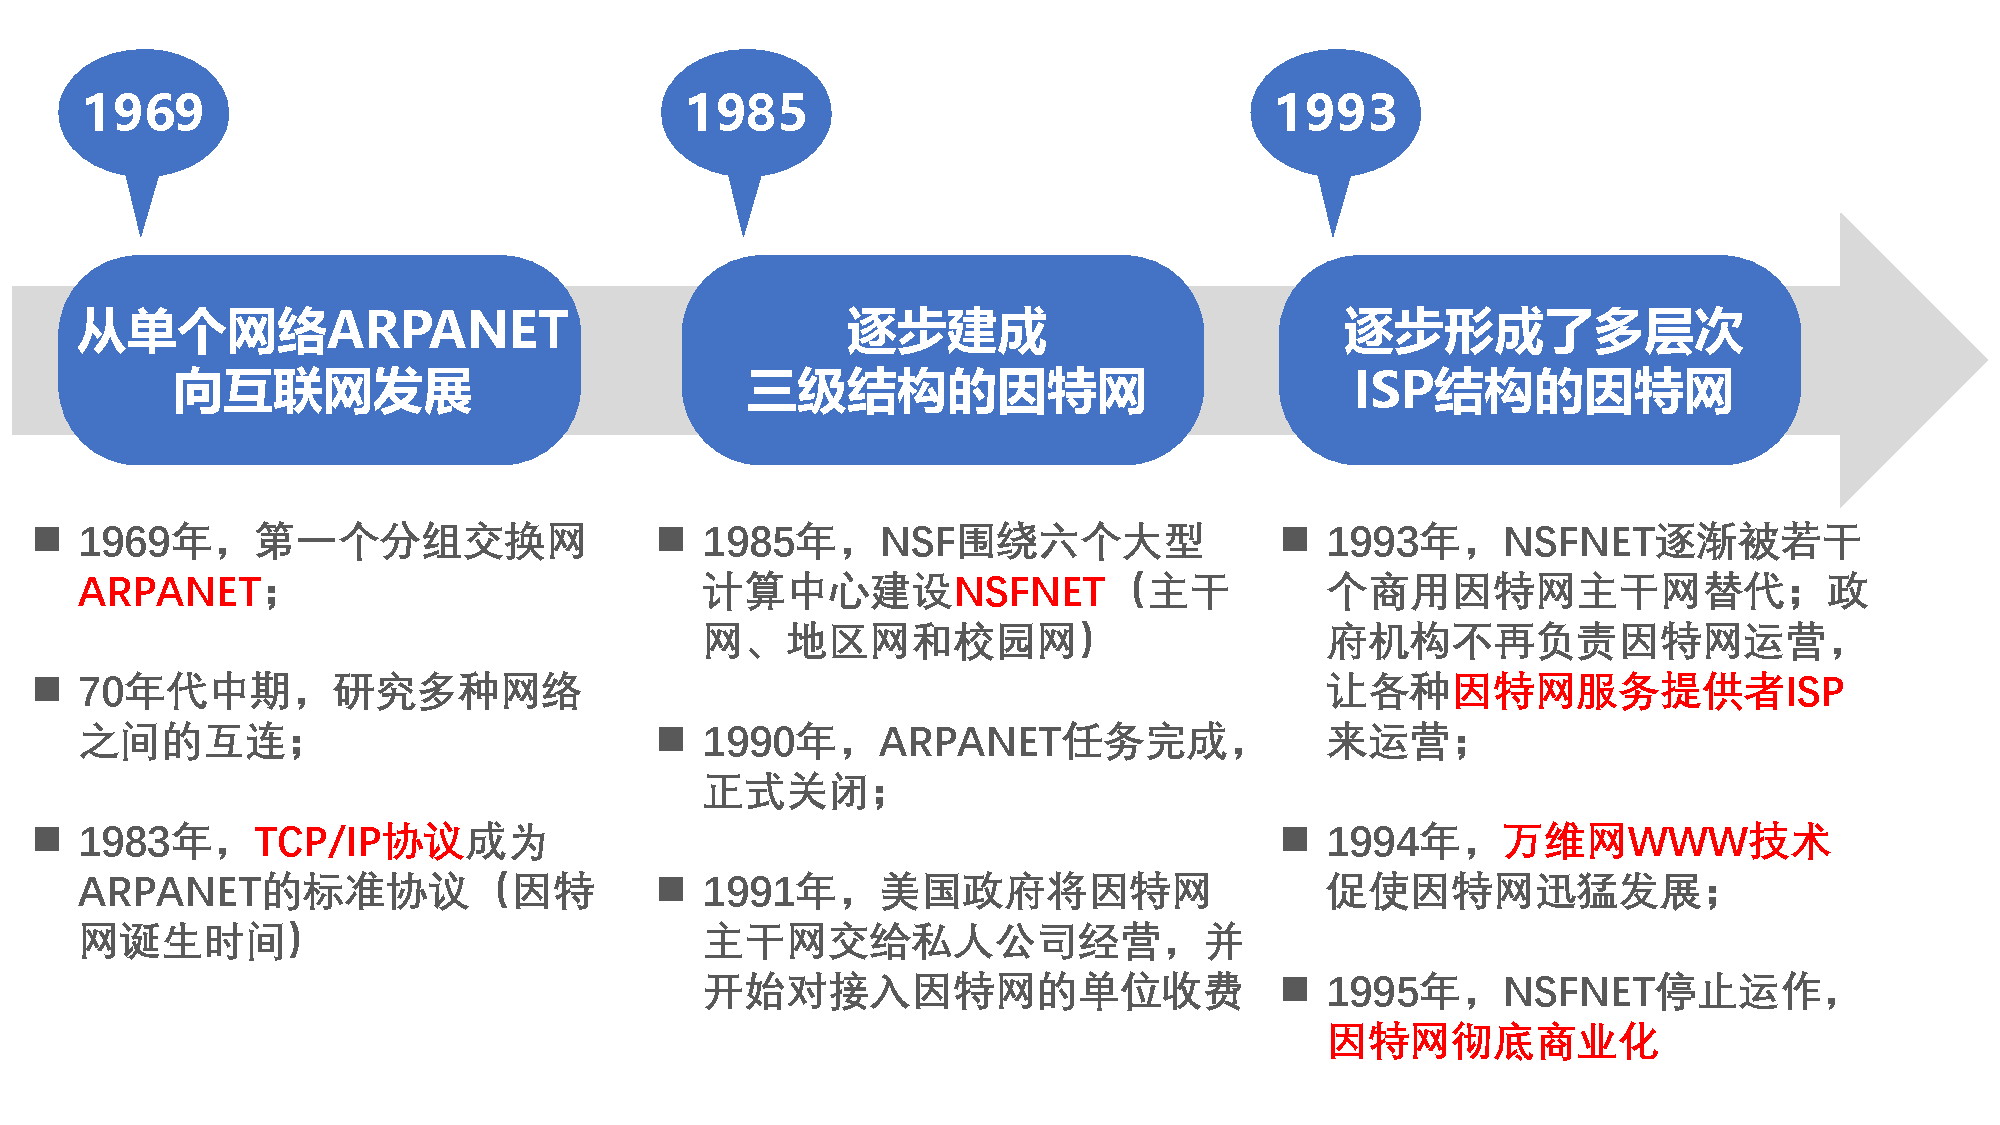
\includegraphics[width=0.9\textwidth]{img/1.2.2}
	\end{figure}

	internet 和 Internet 的差别:
	\begin{itemize}
		\item internet(互连网)是一个通用名词,它泛指由多个计算机网络互连而成的计算机网络。在这些网络之间的通信协议可以任意选择,不一定非要使用 TCP/IP 协议
		\item Internet(互联网,或因特网)是一个专用名词,它指当前全球最大的、开放的、由众多网络相互连接而成的特定互连网,它采用 TCP/IP 协议族作为通信的规则,且其前身是美国的ARPANET
	\end{itemize}

	\begin{figure}[H]
		\centering
		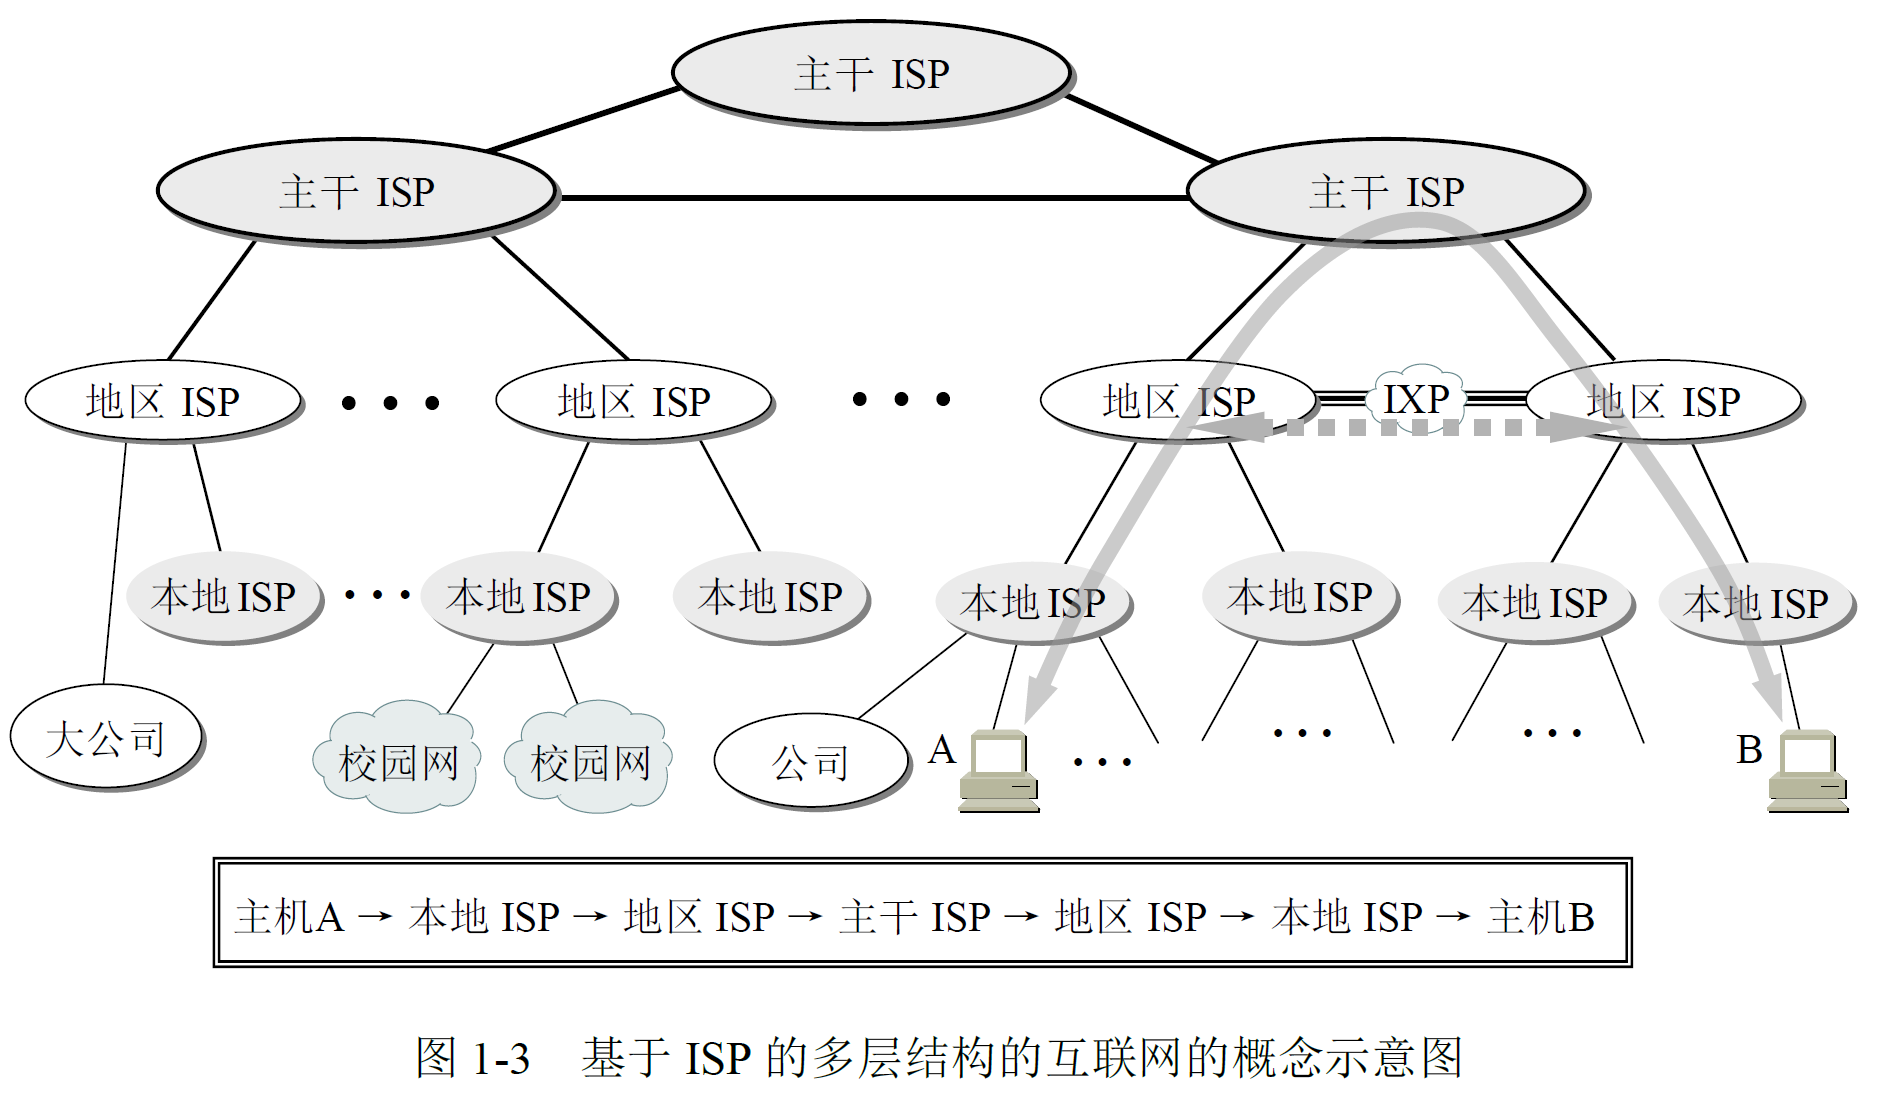
\includegraphics[width=0.75\textwidth]{img/1.3}
	\end{figure}

	\subsection{互联网的标准化工作}
	因特网的标准化工作对因特网的发展起到了非常重要的作用

	因特网在制定其标准上的一个很大的特点是面向公众
	\begin{itemize}
		\item 因特网所有的RFC(Request For Comments,“请求评论”)技术文档都可从因特网上免费下载
		\item 任何人都可以随时用电子邮件发表对某个文档的意见或建议
	\end{itemize}

	因特网协会 ISOC是一个国际性组织,它负责对因特网进行全面管理,以及在世界范围内促进其发展和使用
	\begin{itemize}
		\item 因特网体系结构委员会 IAB, 负责管理因特网有关协议的开发
		\item 因特网工程部 IETF ,负责研究中短期工程问题,主要针对协议的开发和标准化
		\item 因特网研究部 IRTF ,从事理论方面的研究和开发一些需要长期考虑的问题
	\end{itemize}

	\begin{figure}[H]
		\centering
		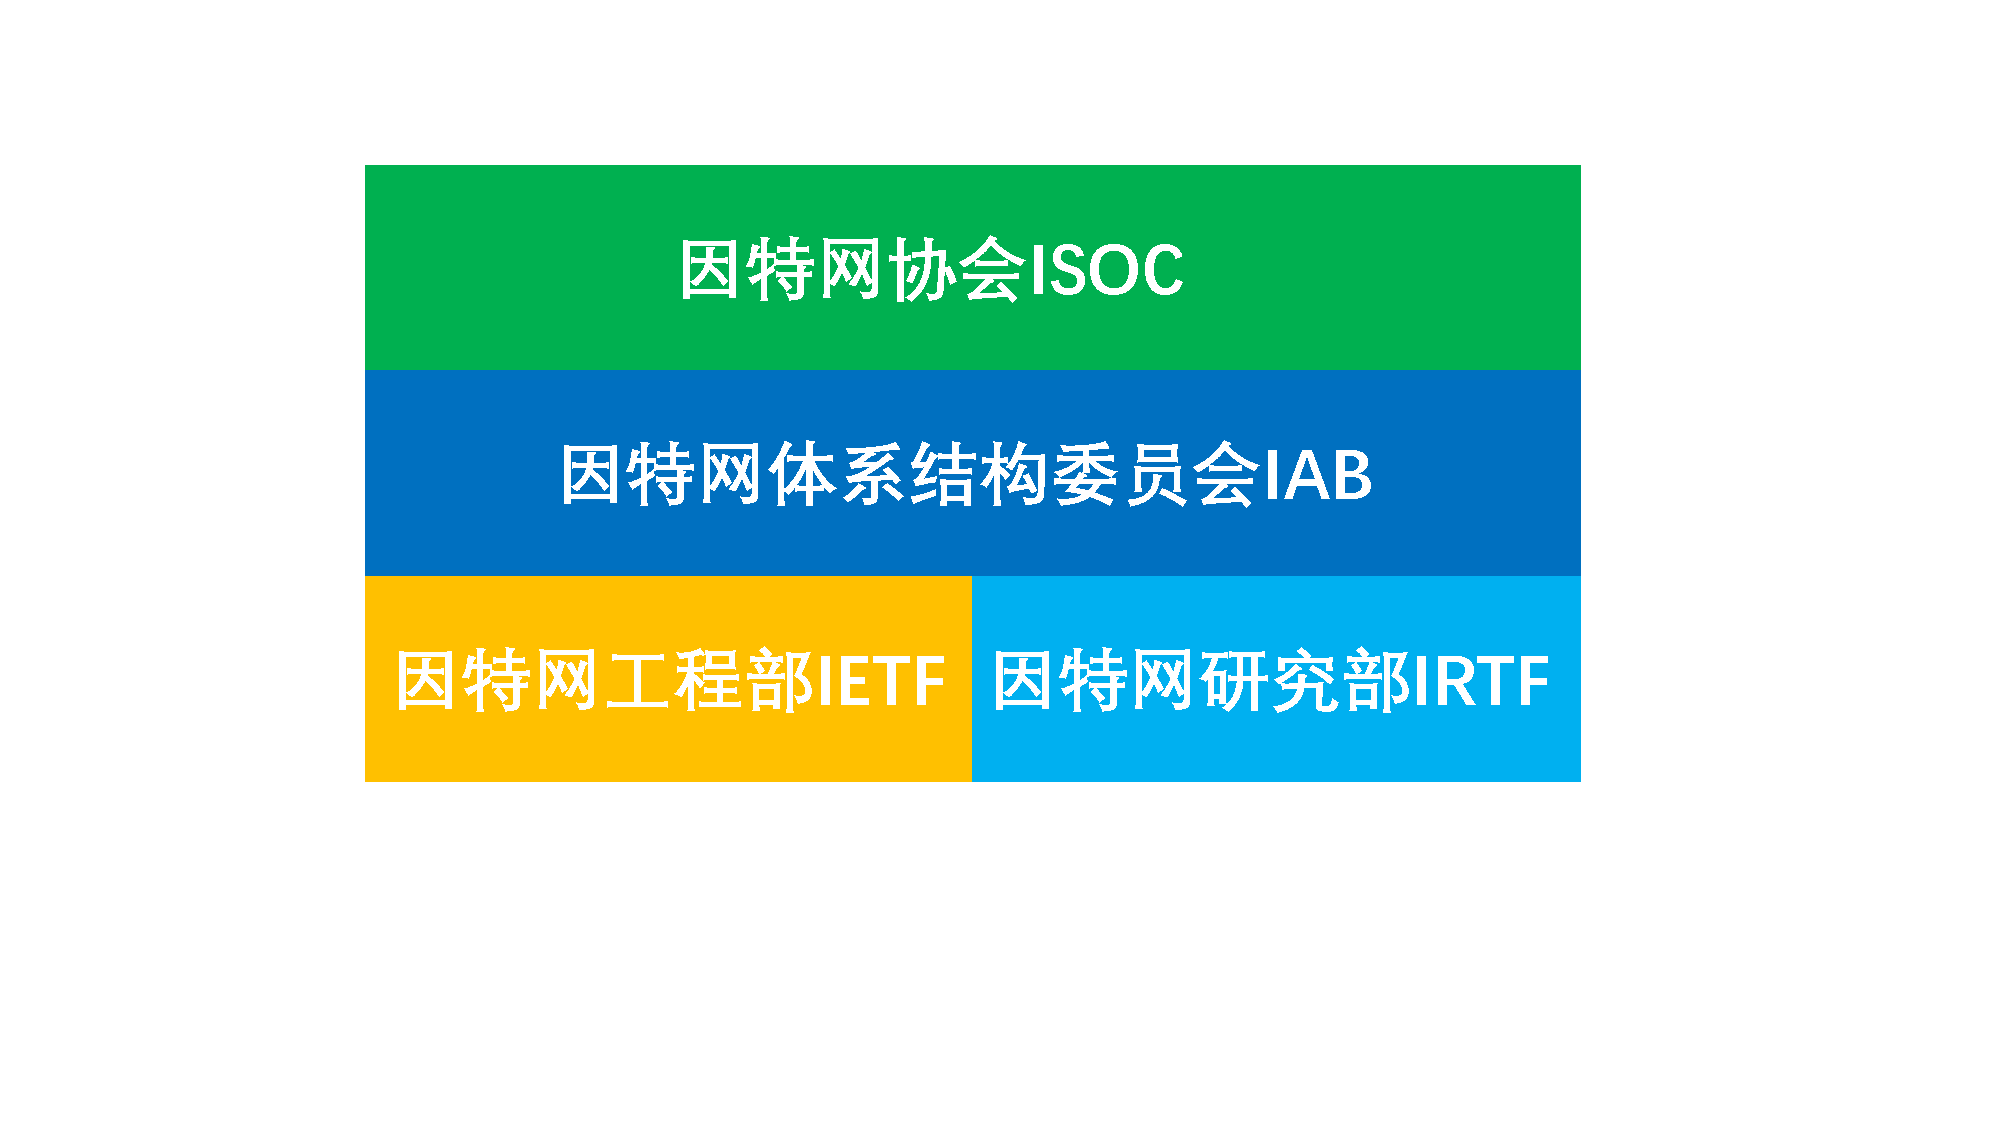
\includegraphics[width=0.4\textwidth]{img/1.2.3}
	\end{figure}
	
	制订因特网的正式标准要经过以下4个阶段:
	\begin{enumerate}[label=\arabic*.]
		\item 因特网草案(在这个阶段还不是RFC文档)
		\item 建议标准(从这个阶段开始就成为RFC文档)
		\item 草案标准
		\item 因特网标准
	\end{enumerate}

	\section{互联网的组成}
	互联网的拓扑结构从工作方式上看,可以划分为两大块:边缘部分和核心部分
	\begin{itemize}
		\item 边缘部分:由所有连接在互联网上的主机组成。这部分是用户直接使用的,用来进行通信(传送数据、音频或视频)和资源共享
		\item 核心部分:由大量网络和连接这些网络的路由器组成。这部分是为边缘部分提供服务的(提供连通性和交换)
	\end{itemize}

	\begin{figure}[H]
		\centering
		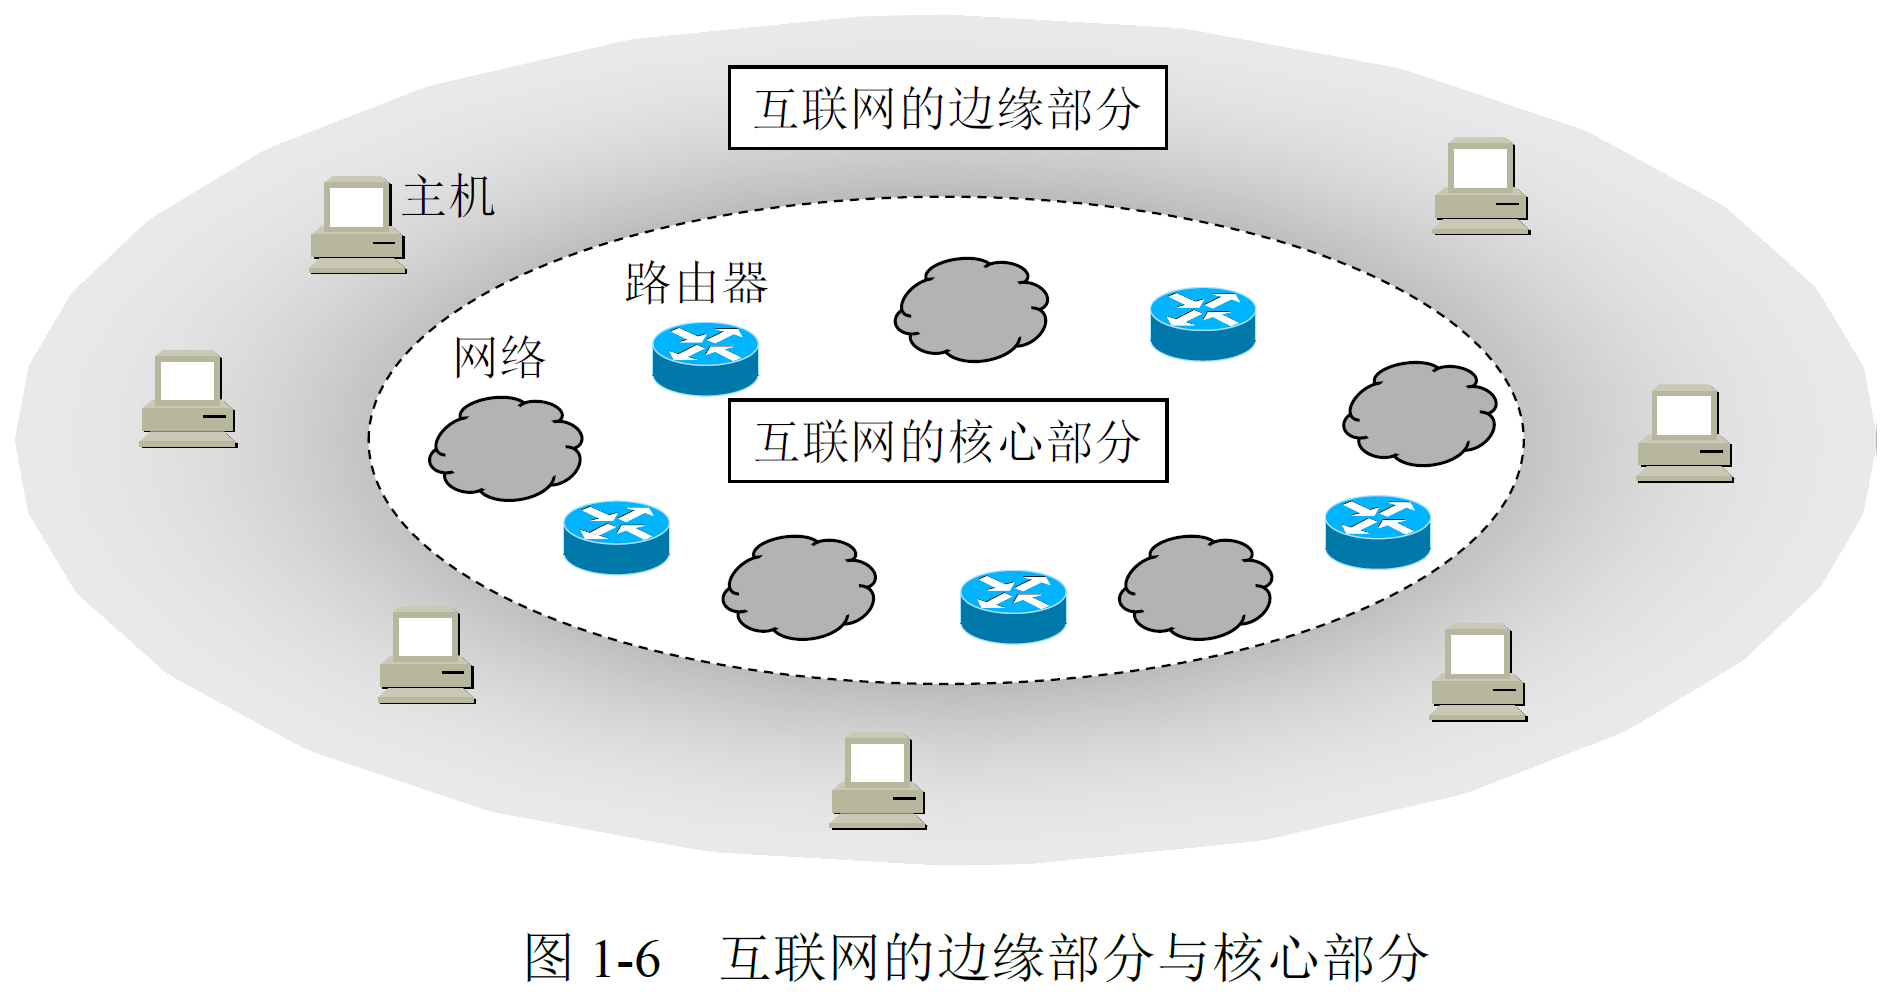
\includegraphics[width=0.6\textwidth]{img/1.6}
	\end{figure}

	\subsection{互联网的边缘部分}
	\begin{itemize}
		\item 处在互联网边缘的部分就是连接在互联网上的所有的主机。这些主机又称为端系统
		\item “主机 A 和主机 B 进行通信”指的是“主机 A 的某个进程和主机 B 上的另一个进程进行通信”,简称为“计算机之间通信”
		\item 在网络边缘的端系统之间的通信方式分为:客户-服务器方式(C/S 方式)和对等方式(P2P 方式)
	\end{itemize}

	\subsubsection{客户-服务器方式}
	\begin{figure}[H]
		\centering
		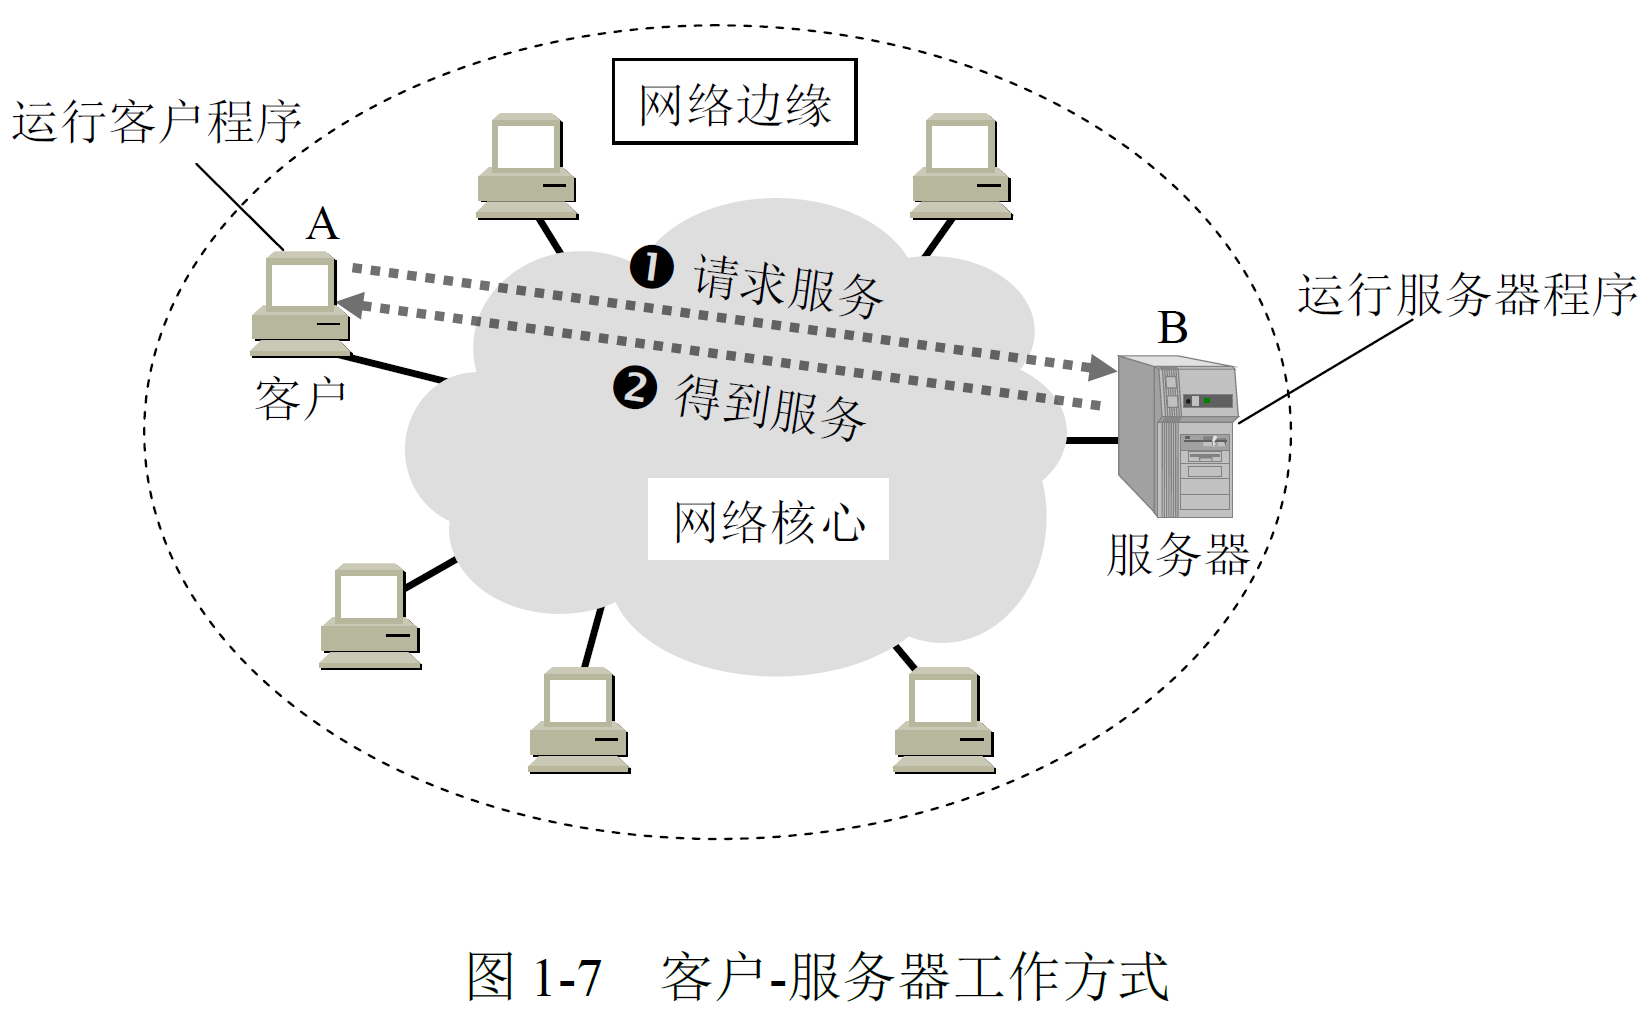
\includegraphics[width=0.6\textwidth]{img/1.7}
	\end{figure}
	\begin{itemize}
		\item 客户(client)和服务器(server)都是指通信中所涉及的两个应用进程,客户-服务器方式所描述的是进程之间服务和被服务的关系
		\item 最主要的特征是:客户是服务请求方,服务器是服务提供方
		\item 服务请求方和服务提供方都要使用网络核心部分所提供的服务
	\end{itemize}

	在实际应用中,客户程序和服务器程序通常还具有以下一些主要特点:
	\begin{itemize}
		\item 客户程序:
		\begin{itemize}
			\item 被用户调用后运行,在通信时主动向远地服务器发起通信(请求服务)。因此,客户程序必须知道服务器程序的地址
			\item 不需要特殊的硬件和很复杂的操作系统
		\end{itemize}
		\item 服务器程序:
		\begin{itemize}
			\item 是一种专门用来提供某种服务的程序,可同时处理多个远地或本地客户的请求
			\item 系统启动后即自动调用并一直不断地运行着,被动地等待并接受来自各地的客户的通信请求。因此,服务器程序不需要知道客户程序的地址
			\item 一般需要有强大的硬件和高级的操作系统支持
		\end{itemize}
		\item 客户与服务器的通信关系建立后,通信可以是双向的,客户和服务器都可发送和接收数据
	\end{itemize}

	\subsubsection{对等连接方式}
	\begin{figure}[H]
		\centering
		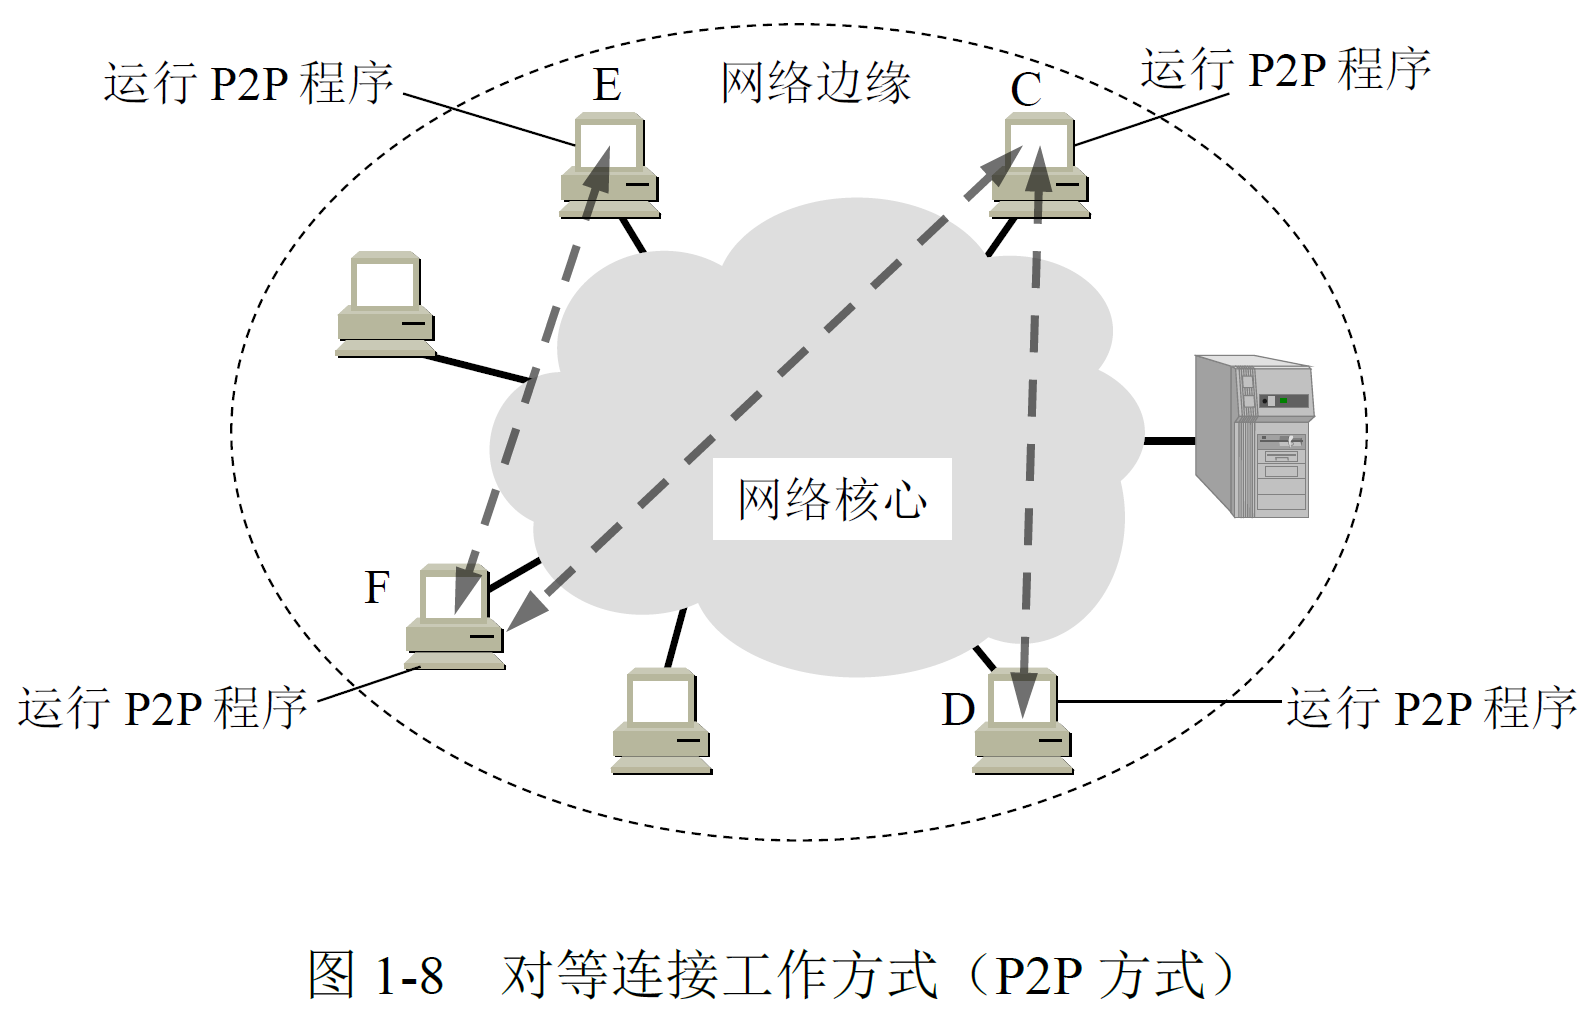
\includegraphics[width=0.65\textwidth]{img/1.8}
	\end{figure}
	
	\begin{itemize}
		\item 两台主机在通信时并不区分哪一个是服务请求方哪一个是服务提供方
		\item 只要两台主机都运行了对等连接软件(P2P,peer-to-peer 软件),它们就可以进行平等的、对等连接通信
		\item 这时,双方都可以下载对方已经存储在硬盘中的共享文档
	\end{itemize}

	\subsection{互联网的核心部分}

	\subsubsection{电路交换的主要特点}

	\begin{itemize}
		\item 电话交换机接通电话线的方式称为电路交换
		\item 从通信资源的分配角度来看,交换就是按照某种方式动态地分配传输线路的资源
		\item 电路交换的三个步骤:
		\begin{enumerate}[label=\arabic*.]
			\item 建立连接(分配通信资源)
			\item 通话(一直占用通信资源)
			\item 释放连接(归还通信资源)
		\end{enumerate}
		\item 电路交换的一个重要特点:在通话的全部时间内,通话的两个用户始终占用端到端的通信资源
		\item 当使用电路交换来传送计算机数据时,其线路的传输效率往往很低:计算机数据是突发式地出现在传输线路上的,已被用户占用的通信线路资源在绝大部分时间里都是空闲的
	\end{itemize}

	\begin{figure}[H]
		\centering
		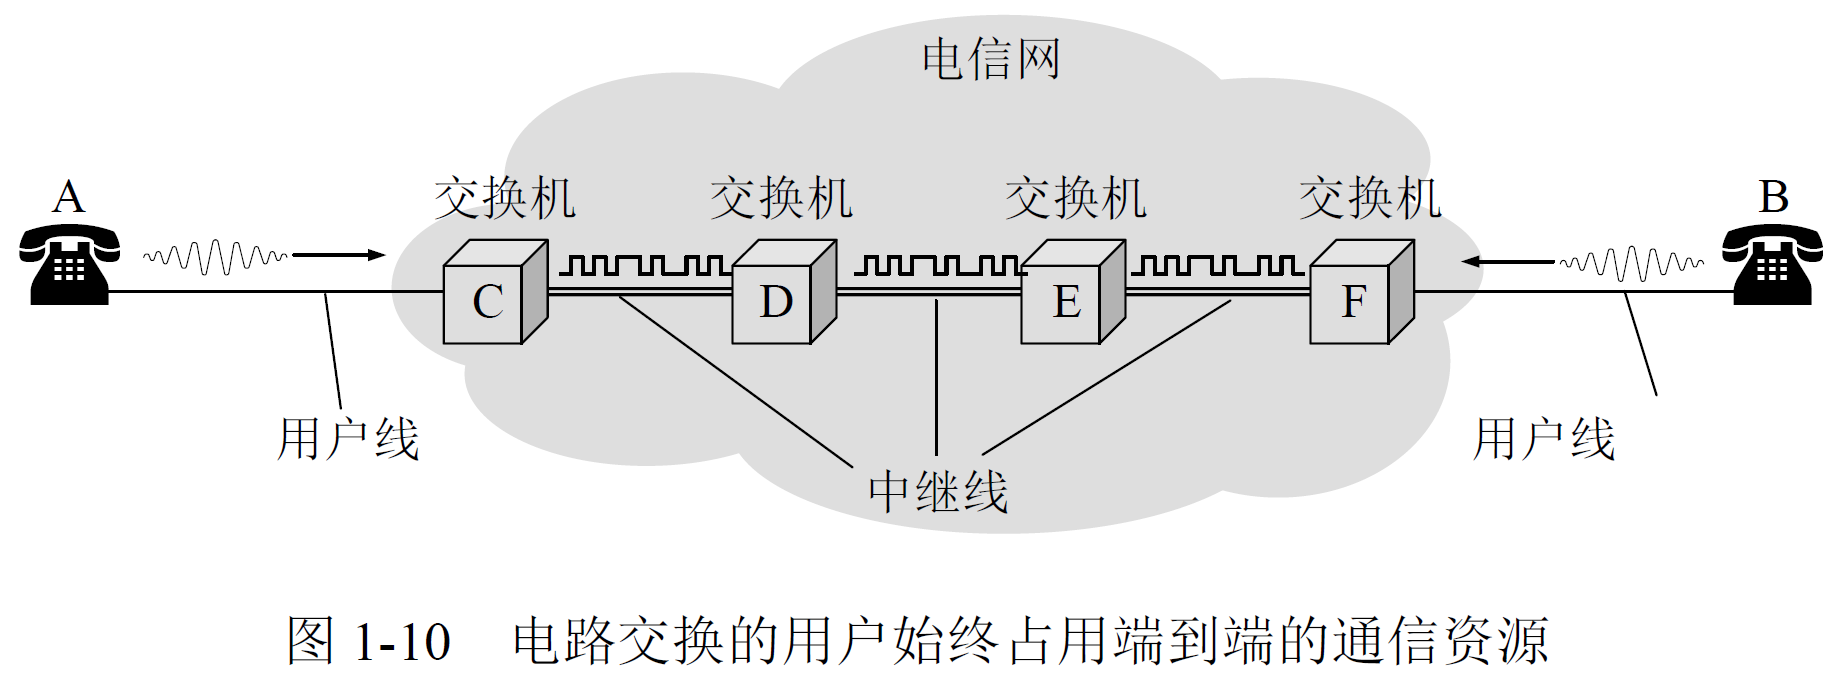
\includegraphics[width=0.85\textwidth]{img/1.10}
	\end{figure}

	\subsubsection{分组交换的主要特点}
	\begin{itemize}
		\item 分组交换采取存储转发技术
		\item 将要发送的整块数据称为一个报文(message)
		\item 在发送报文之前,先把较长的报文划分成为一个个更小的等长数据段,在每一个数据段前面,加上一些由必要的控制信息组成的首部(header)后,就构成了一个分组(packet),又称为“包”,而分组的首部也可称为“包头”
		\item 路由器收到一个分组,先暂时存储一下,检查其首部,查找转发表,按照首部中的目的地址,找到合适的接口转发出去,把分组交给下一个路由器
		\item 如此下去,以存储转发的方式,把分组交付最终的目的主机
		\item 各路由器之间必须经常交换彼此掌握的路由信息,以便创建和动态维护路由器中的转发表,使得转发表能够在整个网络拓扑发生变化时及时更新
	\end{itemize}

	\begin{figure}[H]
		\centering
		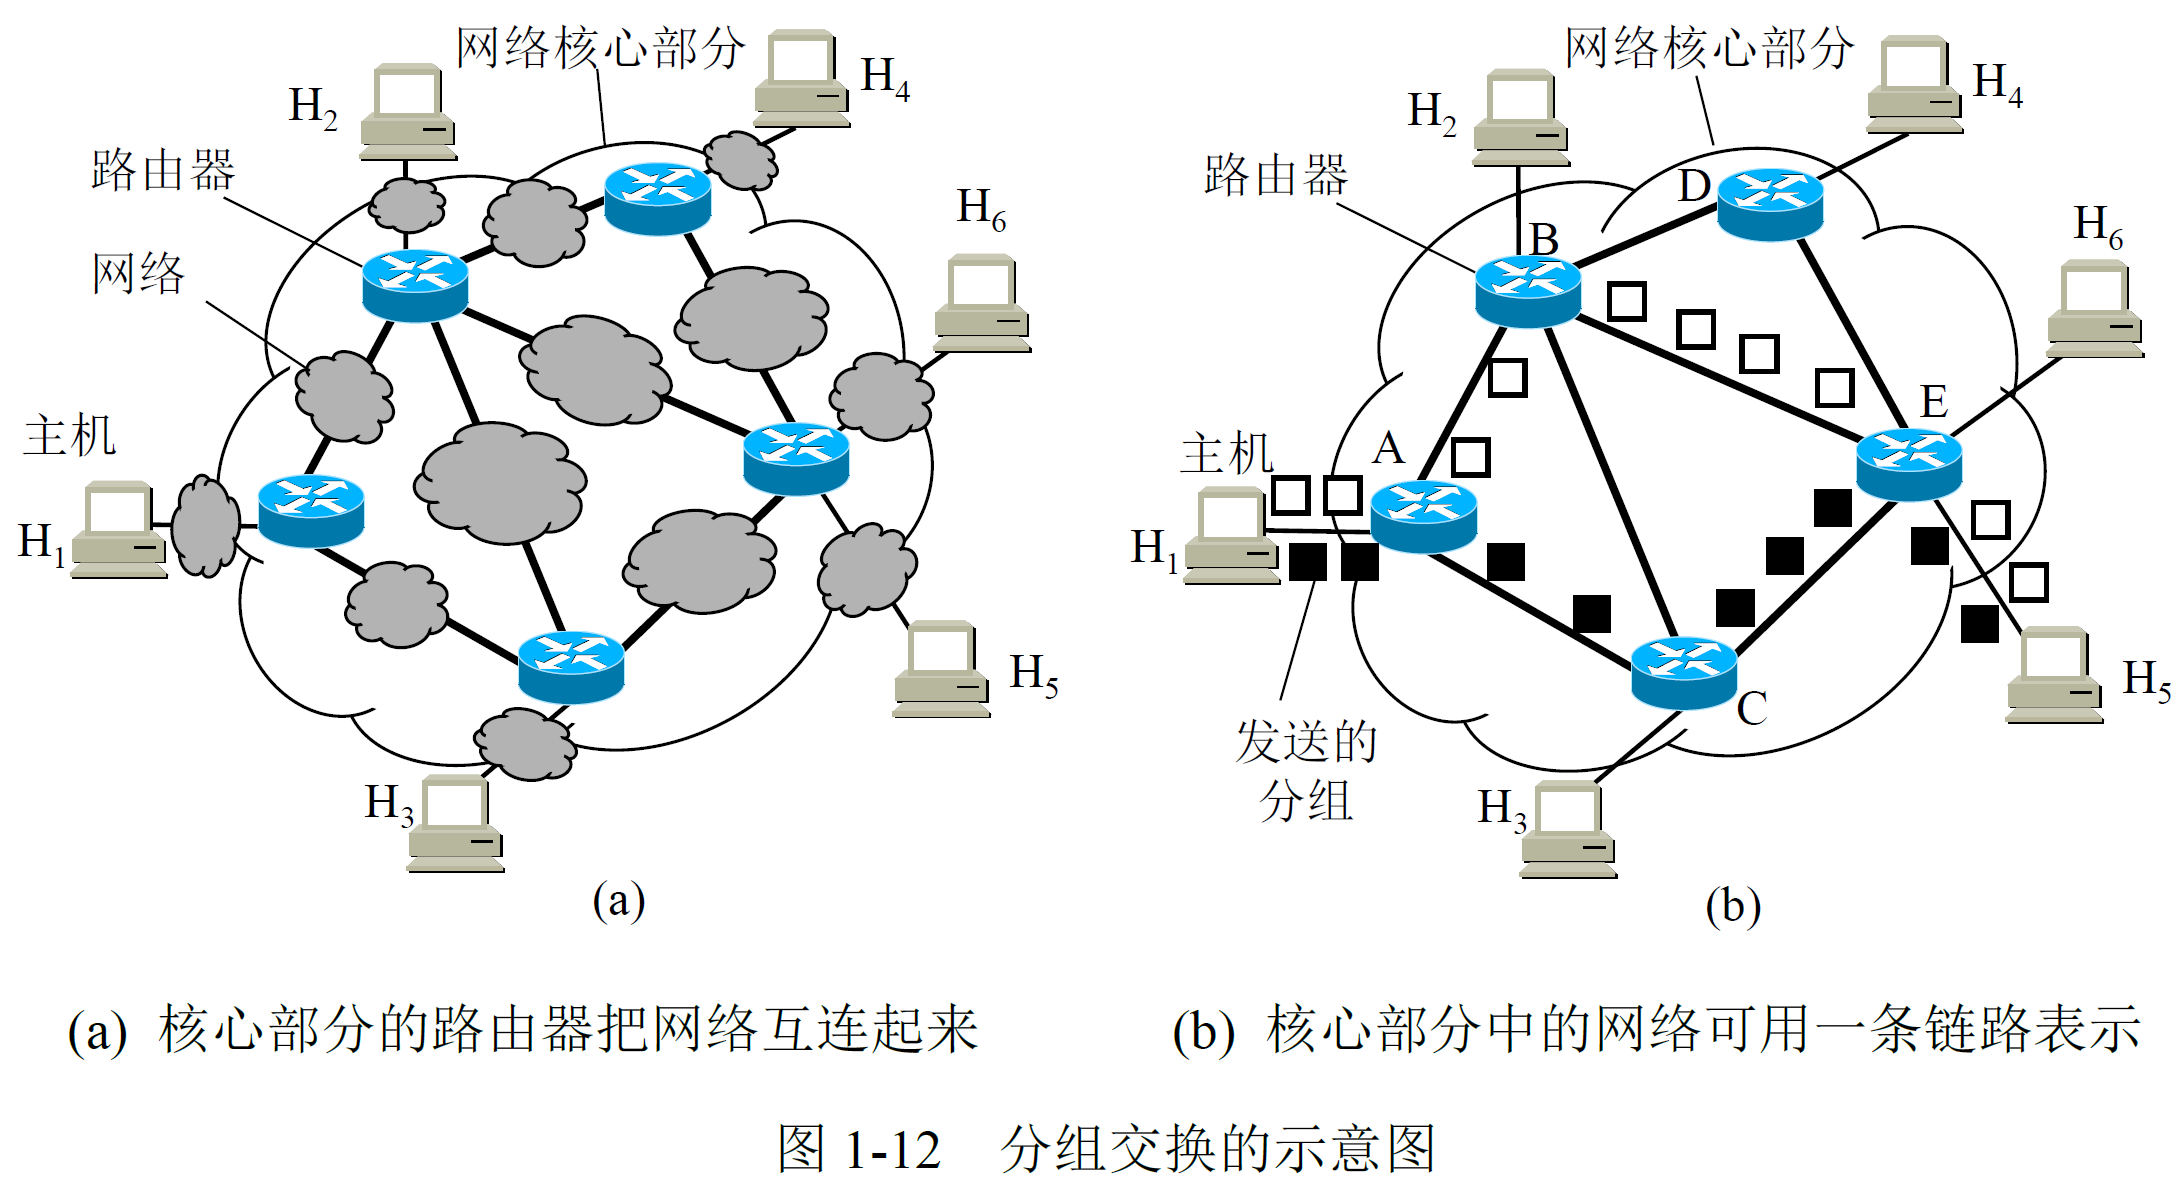
\includegraphics[width=0.8\textwidth]{img/1.12}
	\end{figure}

	分组交换的特点:
	\begin{table}[H]
		\centering
		\begin{tabular}{|c|c|}
		\hline
		优点 & 所采用的手段                             \\ \hline
		高效 & 在分组传输的过程中动态分配传输带宽,对通信链路是逐段占用       \\ \hline
		灵活 & 为每一个分组独立地选择最合适的转发路由                \\ \hline
		迅速 & 以分组作为传送单位,可以不先建立连接就能向其他主机发送分组      \\ \hline
		可靠 & 保证可靠性的网络协议;分布式多路由的分组交换网,使网络有很好的生存性 \\ \hline
		\end{tabular}
	\end{table}

	\subsubsection{电路交换、报文交换和分组交换的对比}
	\begin{figure}[H]
		\centering
		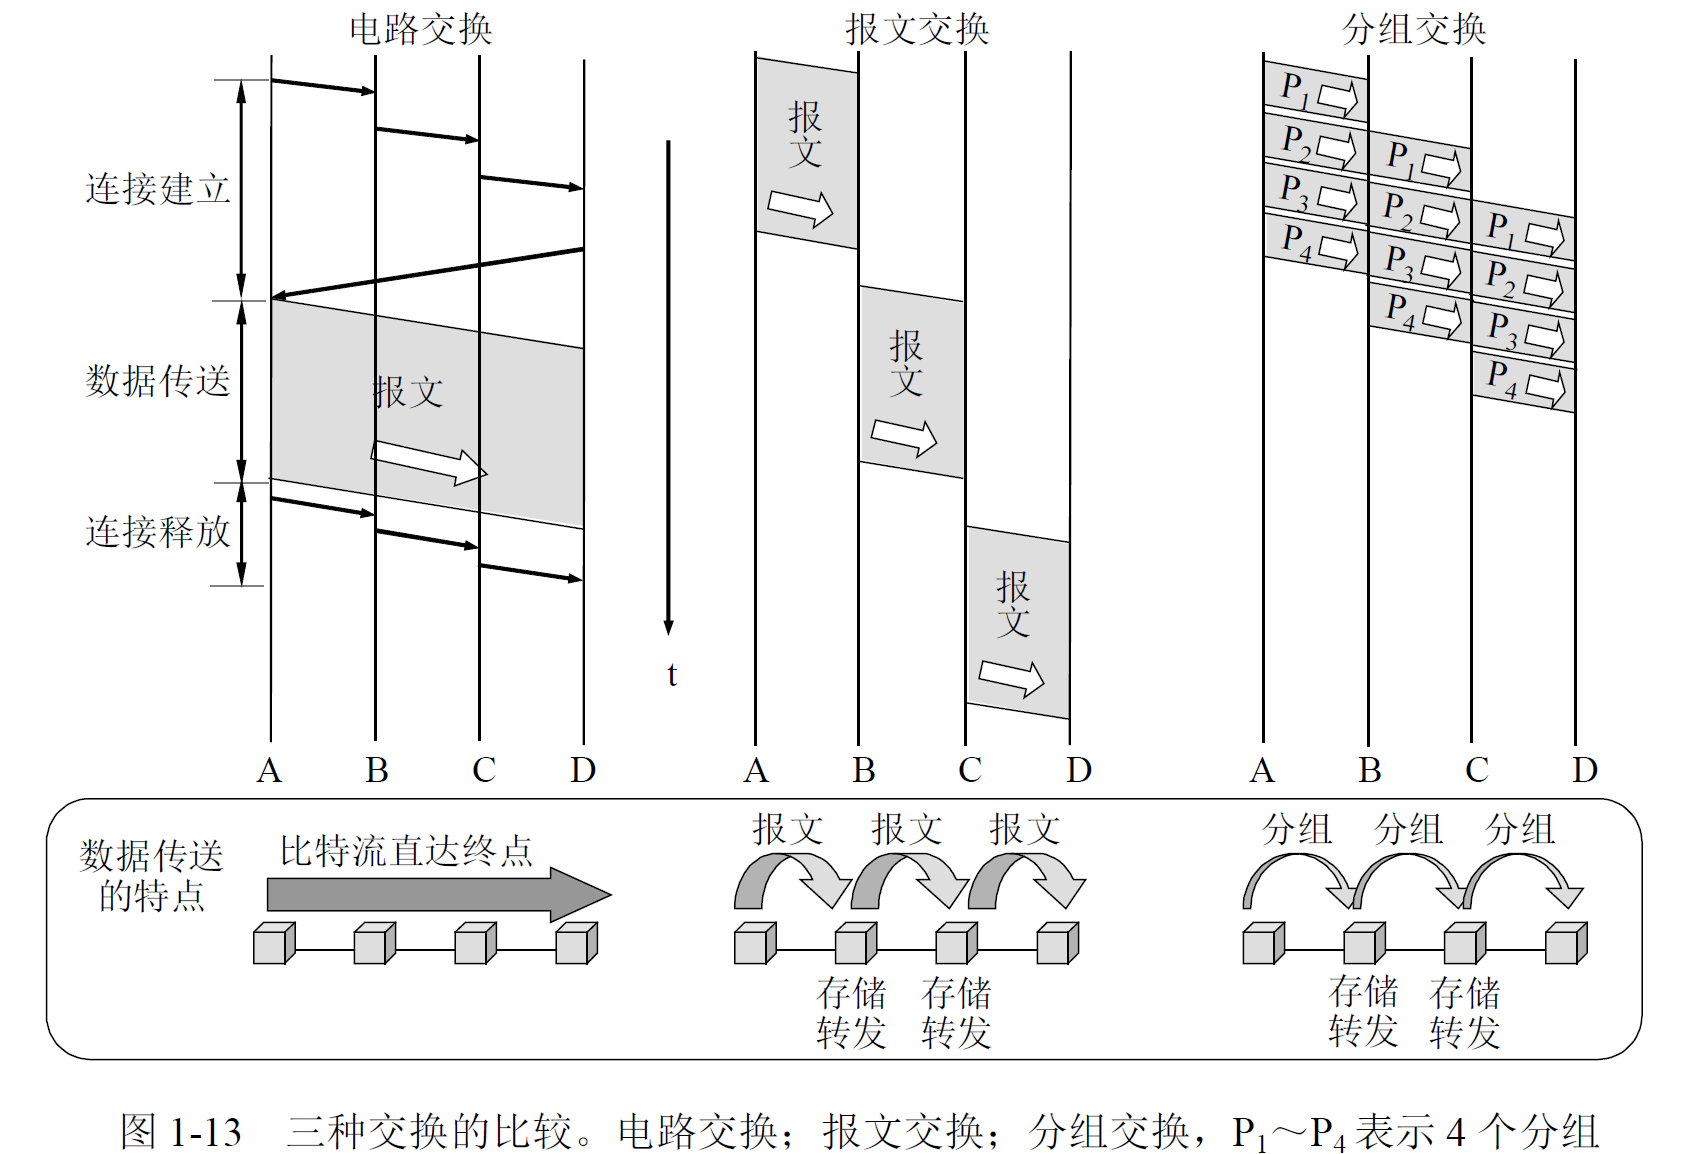
\includegraphics[width=0.8\textwidth]{img/1.13}
	\end{figure}
	\begin{itemize}
		\item 电路交换:整个报文的比特流连续地从源点直达终点,好像在一个管道中传送
		\item 报文交换:整个报文先传送到相邻结点,全部存储下来后查找转发表,转发到下一个结点
		\item 分组交换:单个分组(这只是整个报文的一部分)传送到相邻结点,存储下来后查找转发表,转发到下一个结点
	\end{itemize}

	\section{计算机网络的类别}

	\subsection{计算机网络的定义}
	\begin{itemize}
		\item 计算机网络的精确定义未统一
		\item 计算机网络的最简单定义是:一些互连的、自治的计算机的集合
		\begin{itemize}
			\item 互连:是指计算机之间可以通过有线或者无线的方式进行数据通信
			\item 自治:是指独立的计算机,它有自己的硬件和软件,可以单独运行使用
			\item 集合:是指至少需要两台计算机
		\end{itemize}
		\item 计算机网络的较好的定义是:计算机网络主要是由一些通用的、可编程的硬件互连而成的,而这些硬件并非专门用来实现某一特定目的。这些可编程的硬件能够用来传送多种不同类型的数据,并能支持广泛和日益增长的应用
		\begin{itemize}
			\item 计算机网络所连接的硬件,并不限于一般的计算机,而是包含了智能手机等智能硬件
			\item 计算机网络并非专门用来传输数据,而是能够支持很多种的应用
		\end{itemize}
	\end{itemize}

	\subsection{几种不同类别的计算机网络}
	\begin{table}[H]
		\centering
		\begin{tabular}{|c|c|c|c|c|}
		\hline
		按交换技术分类                                                          & 按使用者分类                                            & 按传输介质分类                                             & 按覆盖范围分类                                                                       & 按拓扑结构分类                                                             \\ \hline
		\begin{tabular}[c]{@{}c@{}}电路交换网络\\ 报文交换网络\\ 分组交换网络\end{tabular} & \begin{tabular}[c]{@{}c@{}}公用网\\ 专用网\end{tabular} & \begin{tabular}[c]{@{}c@{}}有线网络\\ 无线网络\end{tabular} & \begin{tabular}[c]{@{}c@{}}广域网 WAN\\ 城域网 MAN\\ 局域网 LAN\\ 个域网 PAN\end{tabular} & \begin{tabular}[c]{@{}c@{}}总线型网络\\ 星型网络\\ 环型网络\\ 网状型网络\end{tabular} \\ \hline
		\end{tabular}
	\end{table}

	\section{计算机网络的性能}

	\subsection{计算机网络的性能指标}

	\subsubsection{速率}
	表示数据的传送速率,也称为数据率或比特率

	\subsubsection{带宽}
	\begin{itemize}
		\item 本来是指某个信号具有的频带宽度,单位为赫兹。表示某信道允许通过的信号频带范围就称为该信道的带宽(或通频带)
		\item 在计算机网络中,带宽用来表示网络中某通道传送数据的能力,因此网络带宽表示在单位时间内网络中的某信道所能通过的“最高数据率”,单位是“比特每秒”
	\end{itemize}

	\subsubsection{吞吐量}
	吞吐量表示在单位时间内通过某个网络(或信道、接口)的实际的数据量

	\subsubsection{时延}
	时延是指数据(一个报文或分组,甚至比特)从网络(或链路)的一端传送到另一端所需的时间,共由以下四个部分组成:
	\begin{itemize}
		\item 发送时延:主机或路由器发送数据帧所需要的时间
		$$\mbox{发送时延}=\frac{\mbox{数据帧长度}(\mathrm{bit})}{\mbox{发送速率}(\mathrm{bit/s})}$$
		\item 传播时延:电磁波在信道中传播一定的距离需要花费的时间
		$$\mbox{传播时延}=\frac{\mbox{信道长度}\ \mathrm{(m)}}{\mbox{电磁波在信道上的传播速率}\ \mathrm{(m/s)}}$$
		\item 处理时延:主机或路由器在收到分组时要花费一定的时间进行处理,例如分析分组的首部、从分组中提取数据部分、进行差错检验或查找适当的路由等,一般不便于计算
		\item 排队时延:分组在经过网络传输时,要经过许多路由器。但分组在进入路由器后要先在输入队列中排队等待处理。在路由器确定了转发接口后,还要在输出队列中排队等待转发。当网络的通信量很大时会发生队列溢出,使分组丢失,这相当于排队时延为无穷大
	\end{itemize}
	\begin{figure}[H]
		\centering
		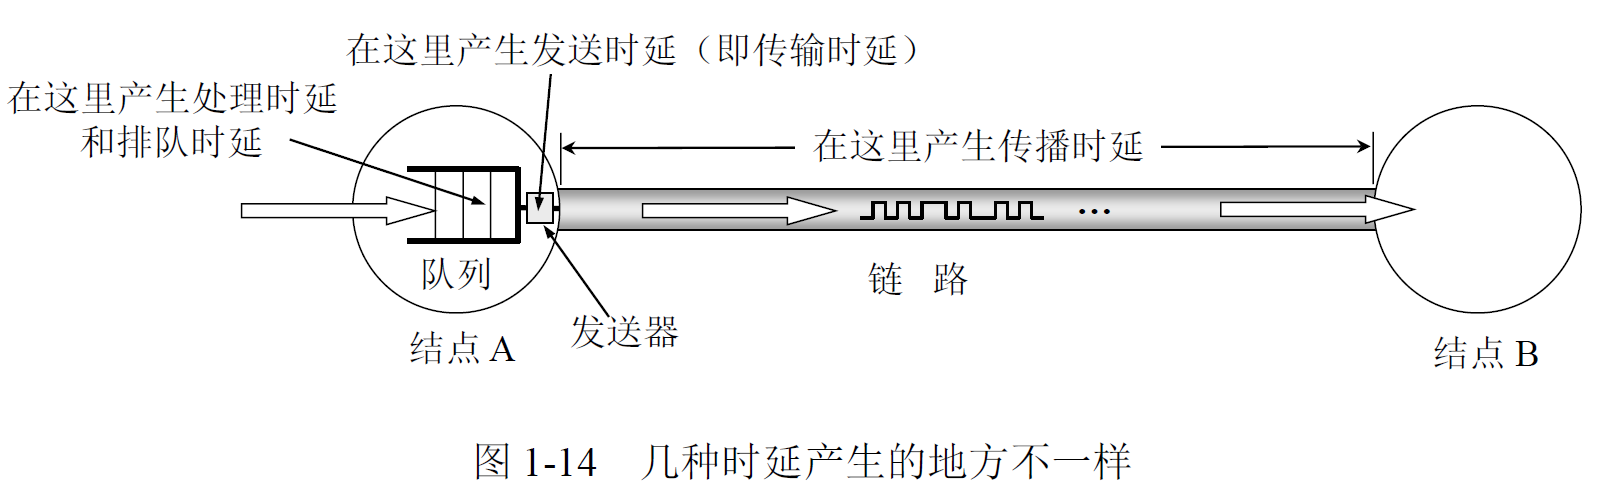
\includegraphics[width=0.9\textwidth]{img/1.14}
	\end{figure}

	\subsubsection{时延带宽积}
	传播时延与带宽的乘积
	\begin{itemize}
		\item 若发送端连续发送数据,则在所发送的第一个比特即将到达终点时,发送端就已经发送了时延带宽积个比特
		\item 链路的时延带宽积又称为以比特为单位的链路长度
	\end{itemize}

	\begin{figure}[H]
		\centering
		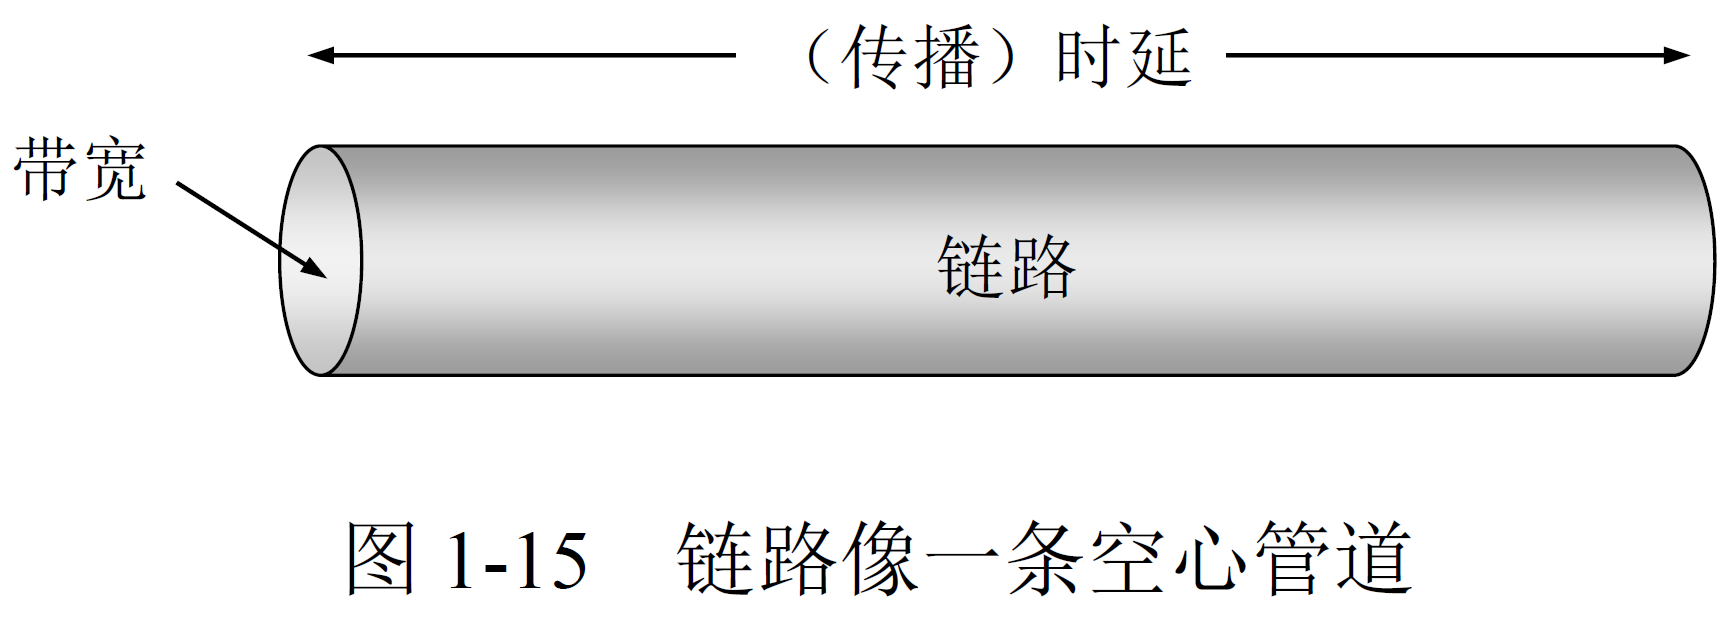
\includegraphics[width=0.4\textwidth]{img/1.15}
	\end{figure}

	\subsubsection{往返时间}
	\begin{itemize}
		\item 在许多情况下,互联网上的信息不仅仅单方向传输,而是双向交互的
		\item 我们有时很需要知道双向交互一次所需的时间
		\item 因此,往返时间 RTT(Round-Trip Time)也是一个重要的性能指标
	\end{itemize}

	\subsubsection{利用率}
	\begin{itemize}
		\item 利用率分为信道利用率和网络利用率
		\begin{itemize}
			\item 信道利用率:表示某信道有百分之几的时间是被利用的(有数据通过)
			\item 网络利用率:全网络的信道利用率的加权平均
		\end{itemize}
		\item 根据排队论,当某信道的利用率增大时,该信道因此的时延也会迅速增加
		\item 信道利用率并非越高越好,一些拥有较大主干网的 ISP 通常控制信道利用率不超过 50\%
		\item 令$D_0$ 表示网络空闲时的时延,$D$表示网络当前的时延,那么在适当的假定条件下,$D$、$D_0$和利用率$U$之间的关系为$$D=\frac{D_0}{1-U}$$
	\end{itemize}

	\subsubsection{丢包率}
	\begin{itemize}
		\item 丢包率即分组丢失率,是指在一定的时间范围内,传输过程中丢失的分组数量与总分组数量的比率
		\item 丢包率具体可分为接口丢包率、结点丢包率、链路丢包率、路径丢包率、网络丢包率等
		\item 丢包率是网络运维人员非常关心的一个网络性能指标,但对普通用户来说往往并不关心这个指标,因为他们通常意识不到网络丢包
		\item 分组丢失主要有两种情况:
		\begin{itemize}
			\item 分组在传输中出现误码,被结点丢弃
			\item 分组到达一台队列已满的分组交换机时被丢弃;在通信量较大时就可能造成
		\end{itemize}
		\item 因此,丢包率反应网络的拥塞情况
	\end{itemize}


	\subsection{计算机网络的非性能特性}
	\begin{multicols}{2}
		\begin{itemize}
			\item 费用
			\item 质量
			\item 标准化
			\item 可靠性
			\item 可扩展性和可升级性
			\item 易于管理和维护
	\end{itemize}
	\end{multicols}

	\section{计算机网络体系结构}

	\subsection{协议与划分层次}
	\begin{itemize}
		\item 在计算机网络中要做到有条不紊地交换数据,就必须遵守一些事先约定好的规则。这些规则明确规定了所交换的数据的格式以及有关的同步问题
		\item 为进行网络中的数据交换而建立的规则、标准或约定称为网络协议,简称为协议,主要由以下三个要素构成:
		\begin{itemize}
			\item 语法:即数据与控制信息的结构或格式
			\item 语义:即需要发出何种控制信息,完成何种动作以及做出何种响应
			\item 同步:即事件实现顺序的详细说明
		\end{itemize}
		\item 分层带来的好处:
		\begin{itemize}
			\item 各层之间是独立的。某一层并不需要知道它的下一层是如何实现的,而仅仅需要知道该层通过层间的接口(即界面)所提供的服务。由于每一层只实现一种相对独立的功能,因而可将一个难以处理的复杂问题分解为若干个较容易处理的更小一些的问题。这样,整个问题的复杂程度就下降了
			\item 灵活性好。当任何一层发生变化时(例如由于技术的变化),只要层间接口关系保持不变,则在这层以上或以下各层均不受影响。此外,对某一层提供的服务还可进行修改。 当某层提供的服务不再需要时,甚至可以将这层取消
			\item 结构上可分割开。各层都可以采用最合适的技术来实现
			\item 易于实现和维护。这种结构使得实现和调试一个庞大而又复杂的系统变得易于处理,因为整个的系统已被分解为若干个相对独立的子系统
			\item 能促进标准化工作。因为每一层的功能及其所提供的服务都已有了精确的说明
		\end{itemize}
		\item 计算机网络的各层及其协议的集合就是网络的体系结构。换种说法,计算机网络的体系结构就是这个计算机网络及其构件所应完成的功能的精确定义
		\item 体系结构是抽象的,而实现则是具体的,是真正在运行的 计算机硬件和软件
	\end{itemize}

	\subsection{具有五层协议的体系结构}
	\begin{figure}[H]
		\centering
		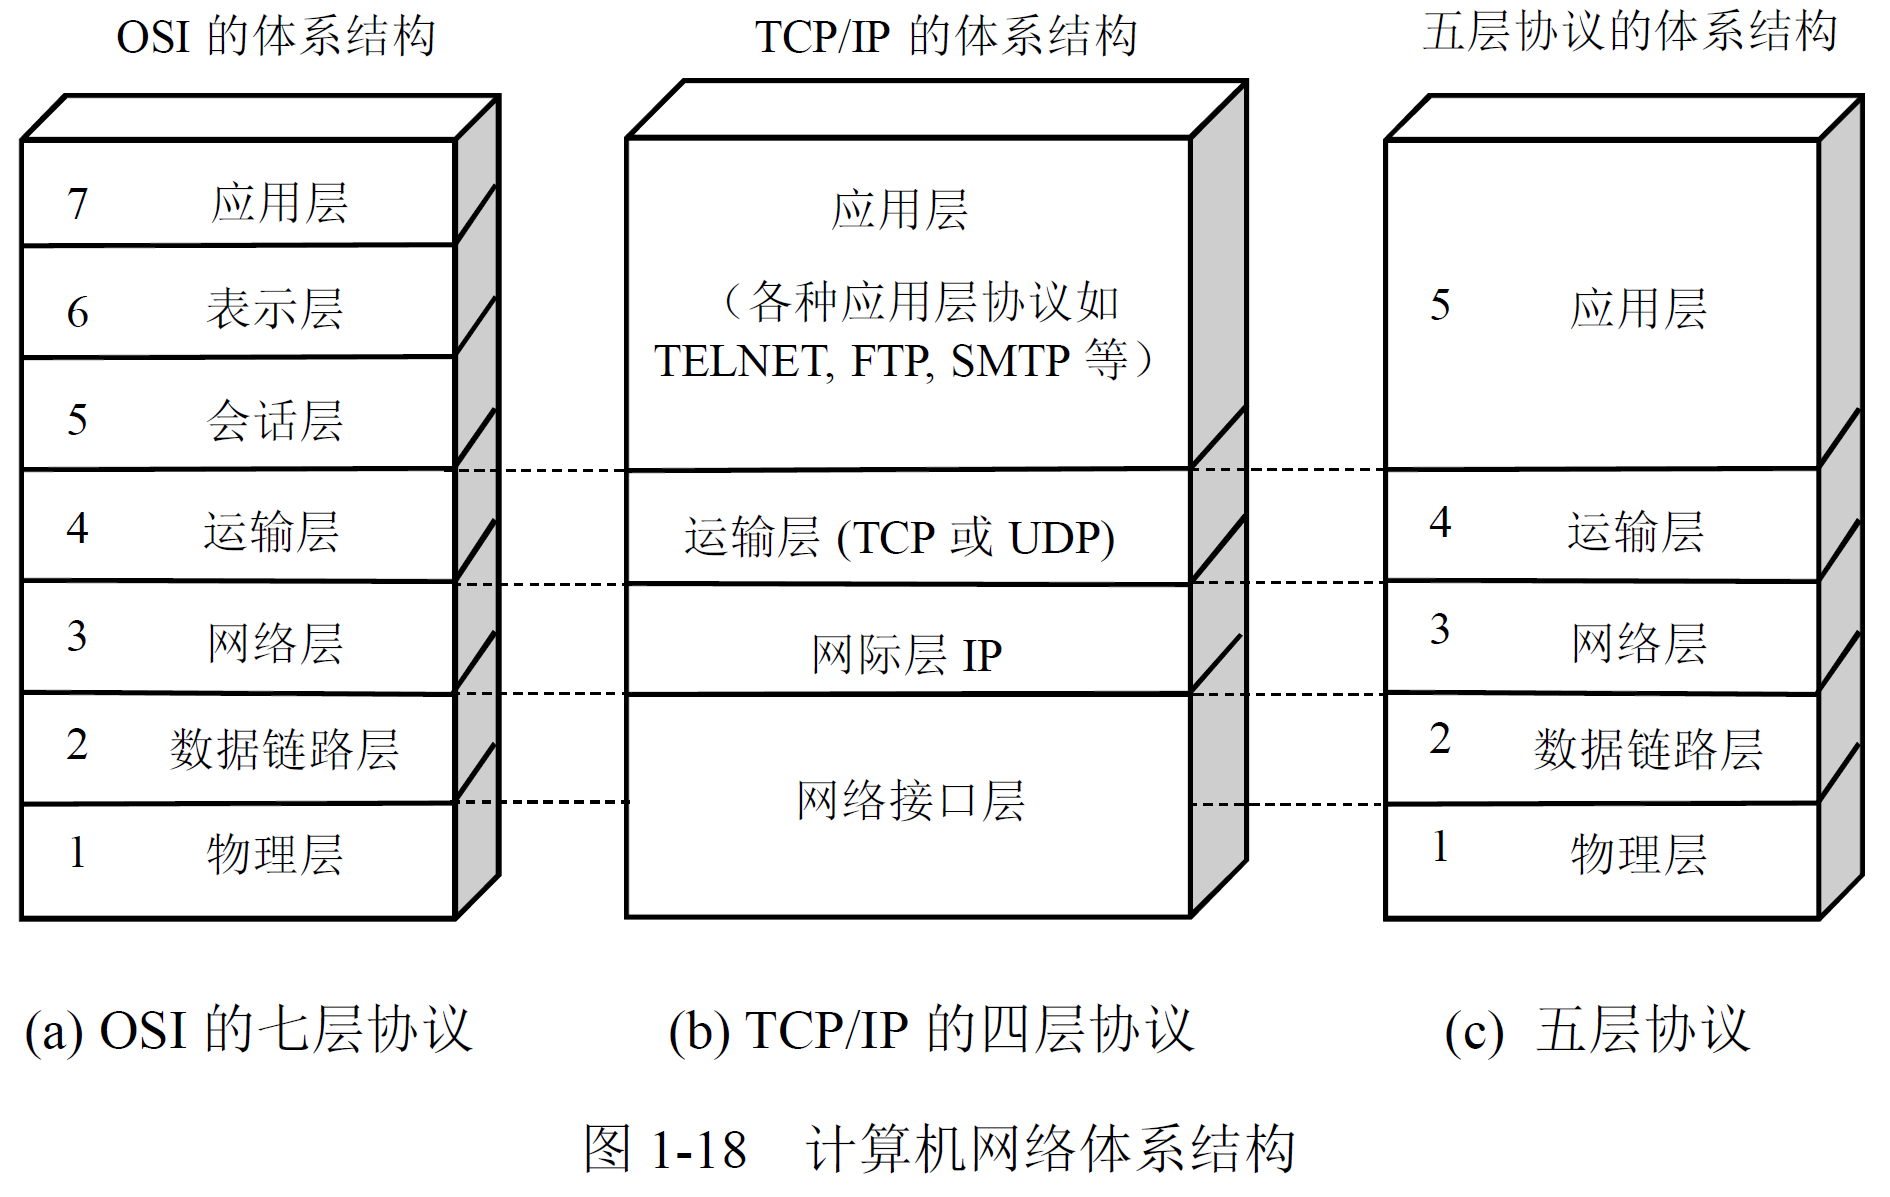
\includegraphics[width=0.85\textwidth]{img/1.18}
	\end{figure}

	\subsubsection{应用层}
	\begin{itemize}
		\item 应用层(application layer)的任务是通过应用进程间的交互来完成特定网络应用
		\item 应用层协议定义的是应用进程间通信和交互的规则
		\item 对于不同的网络应用需要有不同的应用层协议。在互联网中的应用层协议很多,如域名系统 DNS,支持万维网应用的 HTTP 协议,支持电子邮件的 SMTP 协议,等等
		\item 应用层交互的数据单元称为报文
	\end{itemize}

	\subsubsection{运输层}
	\begin{itemize}
		\item 运输层的任务是负责向两台主机中进程之间的通信提供通用的数据传输服务
		\item 由于一台主机可同时运行多个进程,因此运输层有复用和分用的功能
		\begin{itemize}
			\item 复用是多个应用层进程可同时使用下面运输层的服务
			\item 分用是运输层把收到的信息分别交付上面应用层中的相应进程
		\end{itemize}
		\item 运输层主要使用以下两种协议:
		\begin{itemize}
			\item 传输控制协议 TCP (Transmission Control Protocol):提供面向连接的、可靠的数据传输服务,其数据传输的单位是报文段(segment)
			\item 用户数据报协议 UDP(User Datagram Protocol):提供无连接的、尽最大努力的数据传输服务(不保证数据传输的可靠性),其数据传输的单位是用户数据报
		\end{itemize}
	\end{itemize}


	\subsubsection{网络层}
	\begin{itemize}
		\item 网络层负责为分组交换网上的不同主机提供通信服务
		\item 在发送数据时,网络层把运输层产生的报文段或用户数据报封装成分组或包进行传送
		\item 网络层的另一个任务就是要选择合适的路由,使源主机运输层所传下来的分组,能够通过网络中的路由器找到目的主机
	\end{itemize}

	\subsubsection{数据链路层}
	\begin{itemize}
		\item 两台主机之间的数据传输,总是在一段一段的链路上传送的,这就需要使用专门的链路层的协议
		\item 在两个相邻结点之间传送数据时,数 据链路层将网络层交下来的 IP 数据报组装成帧(framing),在两个相邻结点间的链路上传送帧(frame)。每一帧包括数据和必要的控制信息
		\item 在接收数据时,控制信息使接收端能够知道一个帧从哪个比特开始和到哪个比特结束。这样,数据链路层在收到一个帧后,就可从中提取出数据部分,上交给网络层
		\item 控制信息还使接收端能够检测到所收到的帧中有无差错。如发现有差错,数据链路层就简单地丢弃这个出了差错的帧
	\end{itemize}

	\subsubsection{物理层}
	\begin{itemize}
		\item 在物理层(physical layer)传输的数据是比特
		\item 物理层主要解决的问题有
		\begin{itemize}
			\item 采用怎样的传输媒体(介质)
			\item 采用怎样的物理接口
			\item 使用怎样的信号表示比特0或1
		\end{itemize}
	\end{itemize}
	\begin{figure}[H]
		\centering
		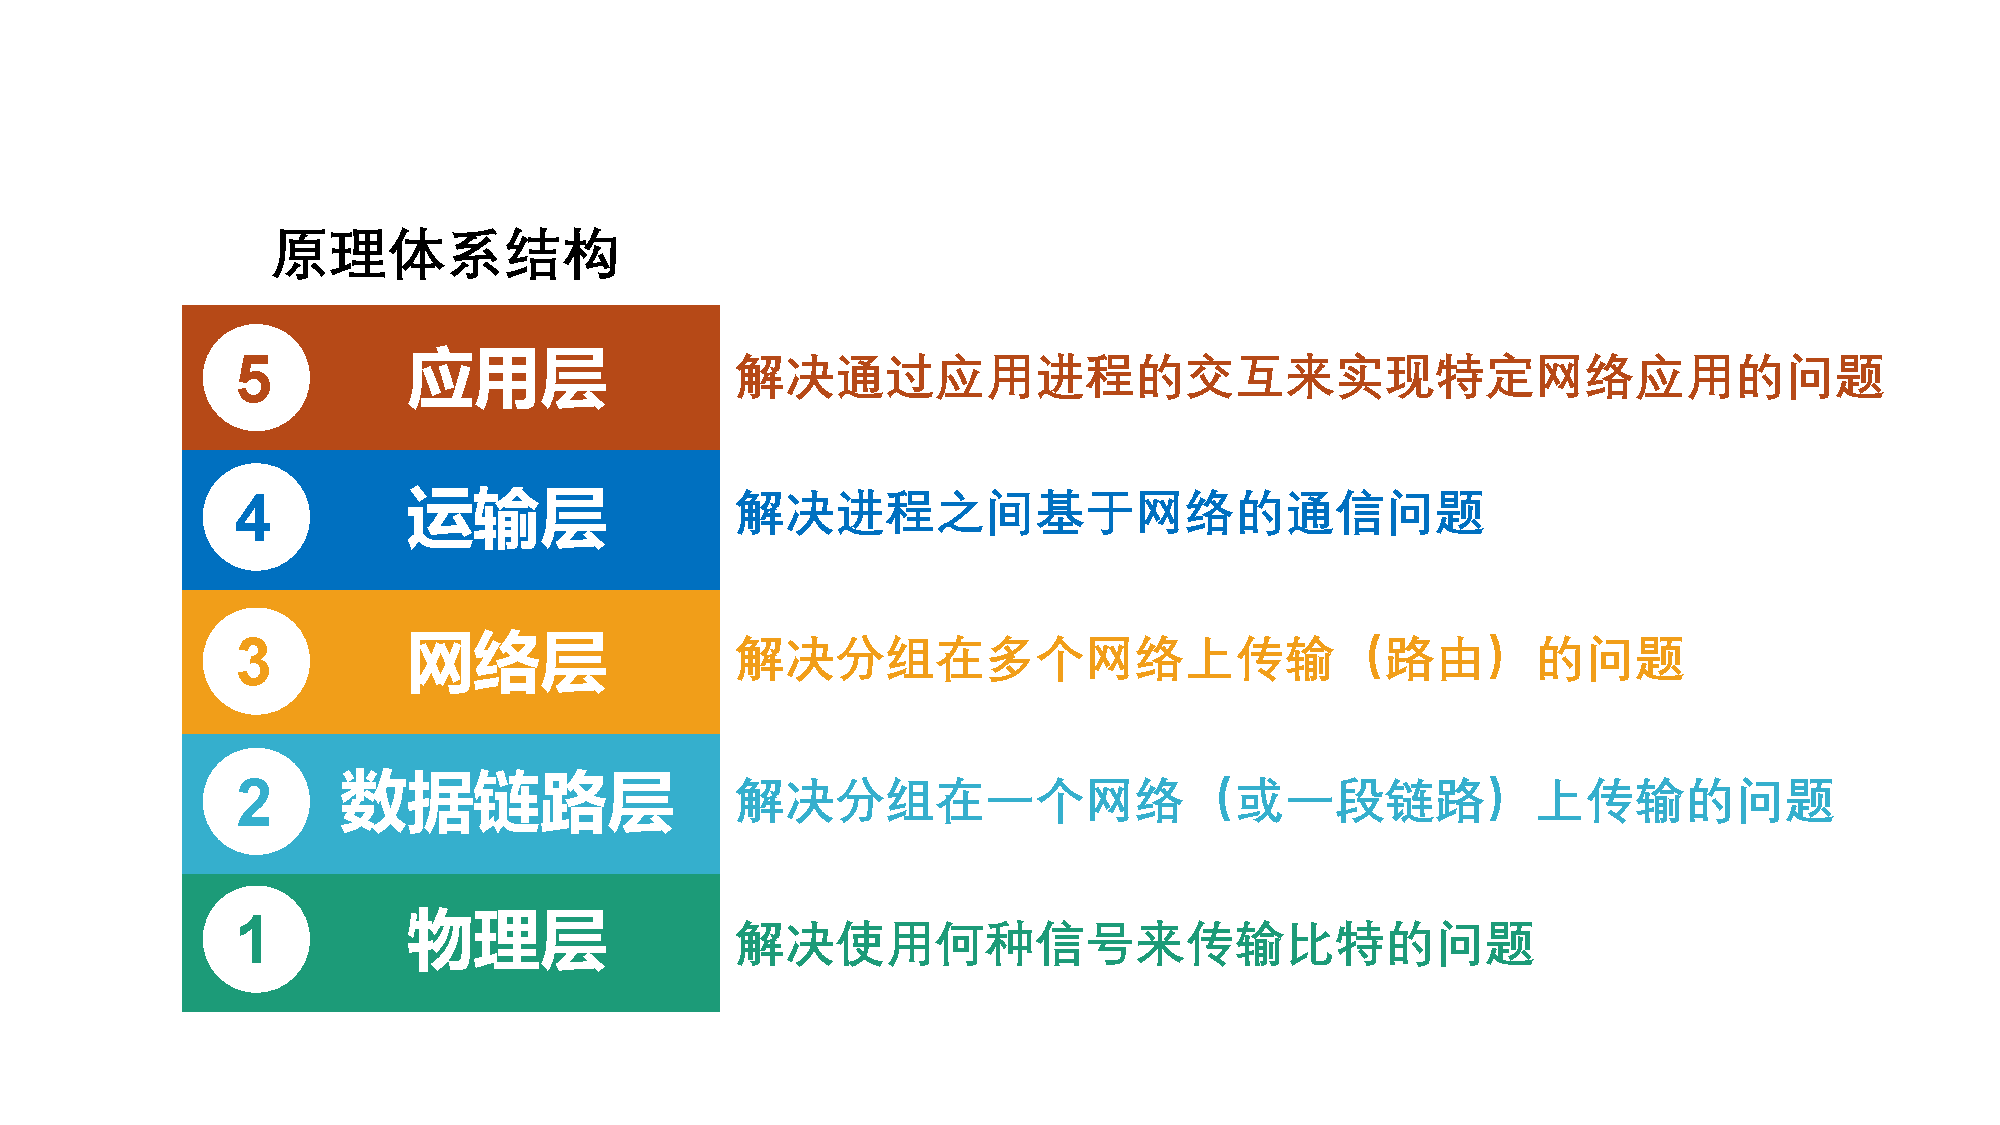
\includegraphics[width=0.75\textwidth]{img/1.6.2}
	\end{figure}

	\subsubsection{数据在各层之间的传递过程}
	\begin{figure}[H]
		\centering
		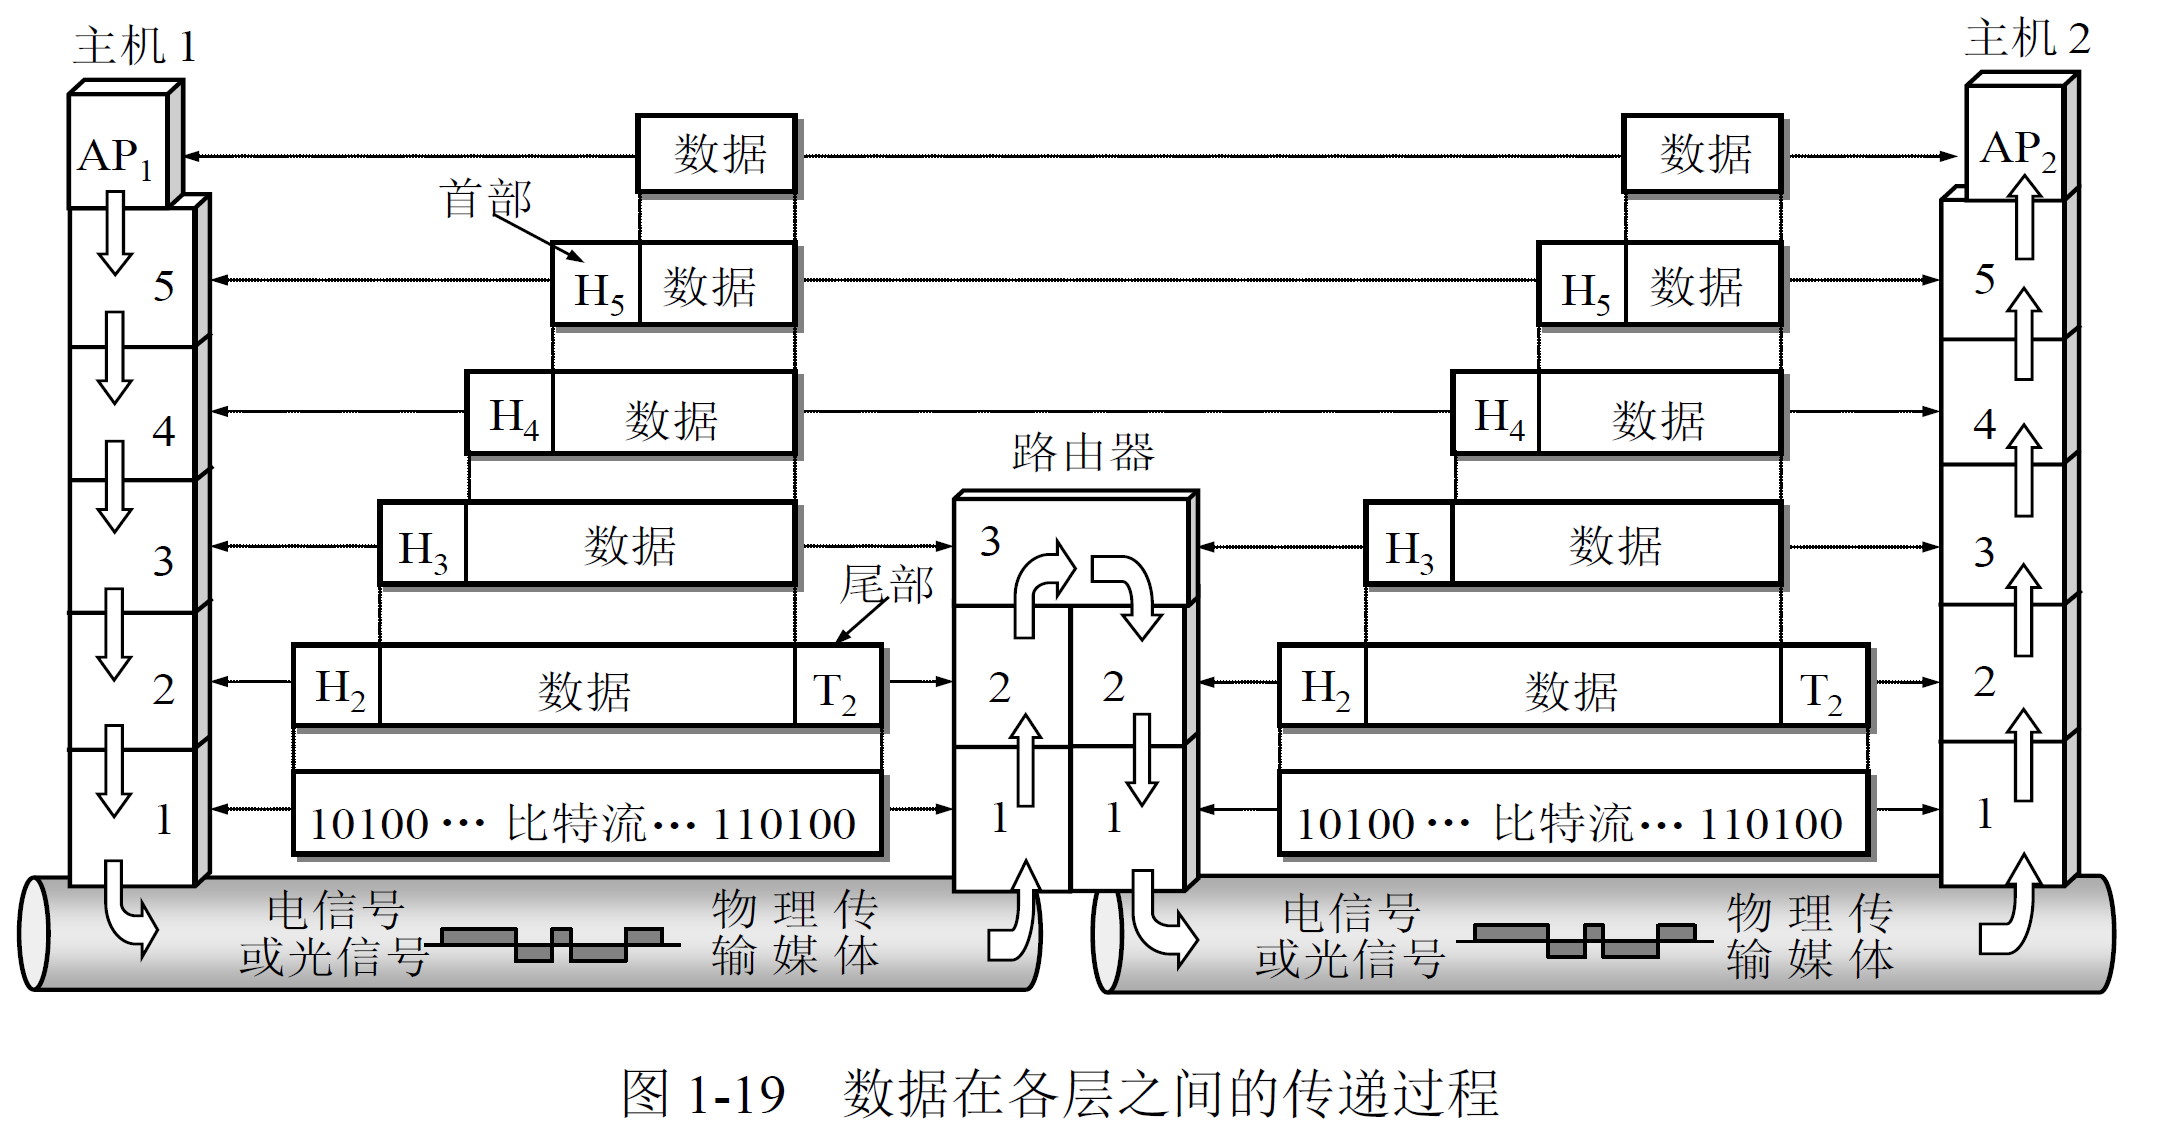
\includegraphics[width=0.85\textwidth]{img/1.19}
	\end{figure}

	\subsection{TCP/IP的体系结构}
	\begin{figure}[H]
		\centering
		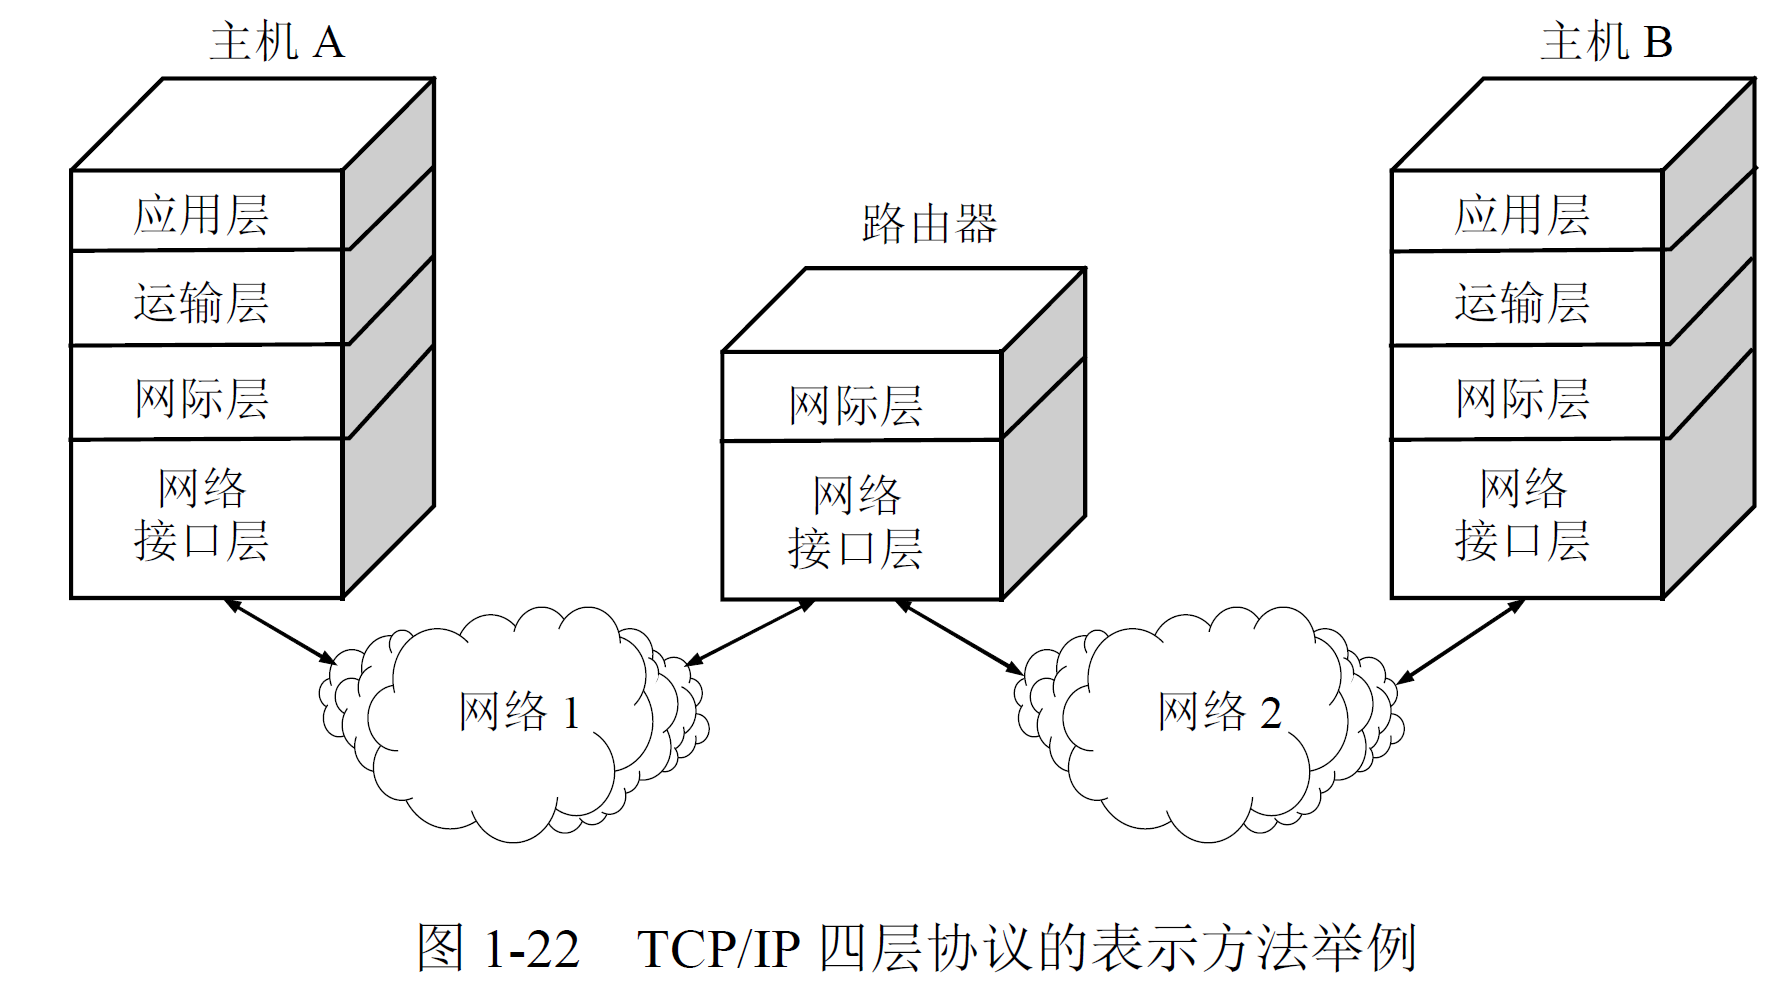
\includegraphics[width=0.65\textwidth]{img/1.22}
	\end{figure}

	\begin{figure}[H]
		\centering
		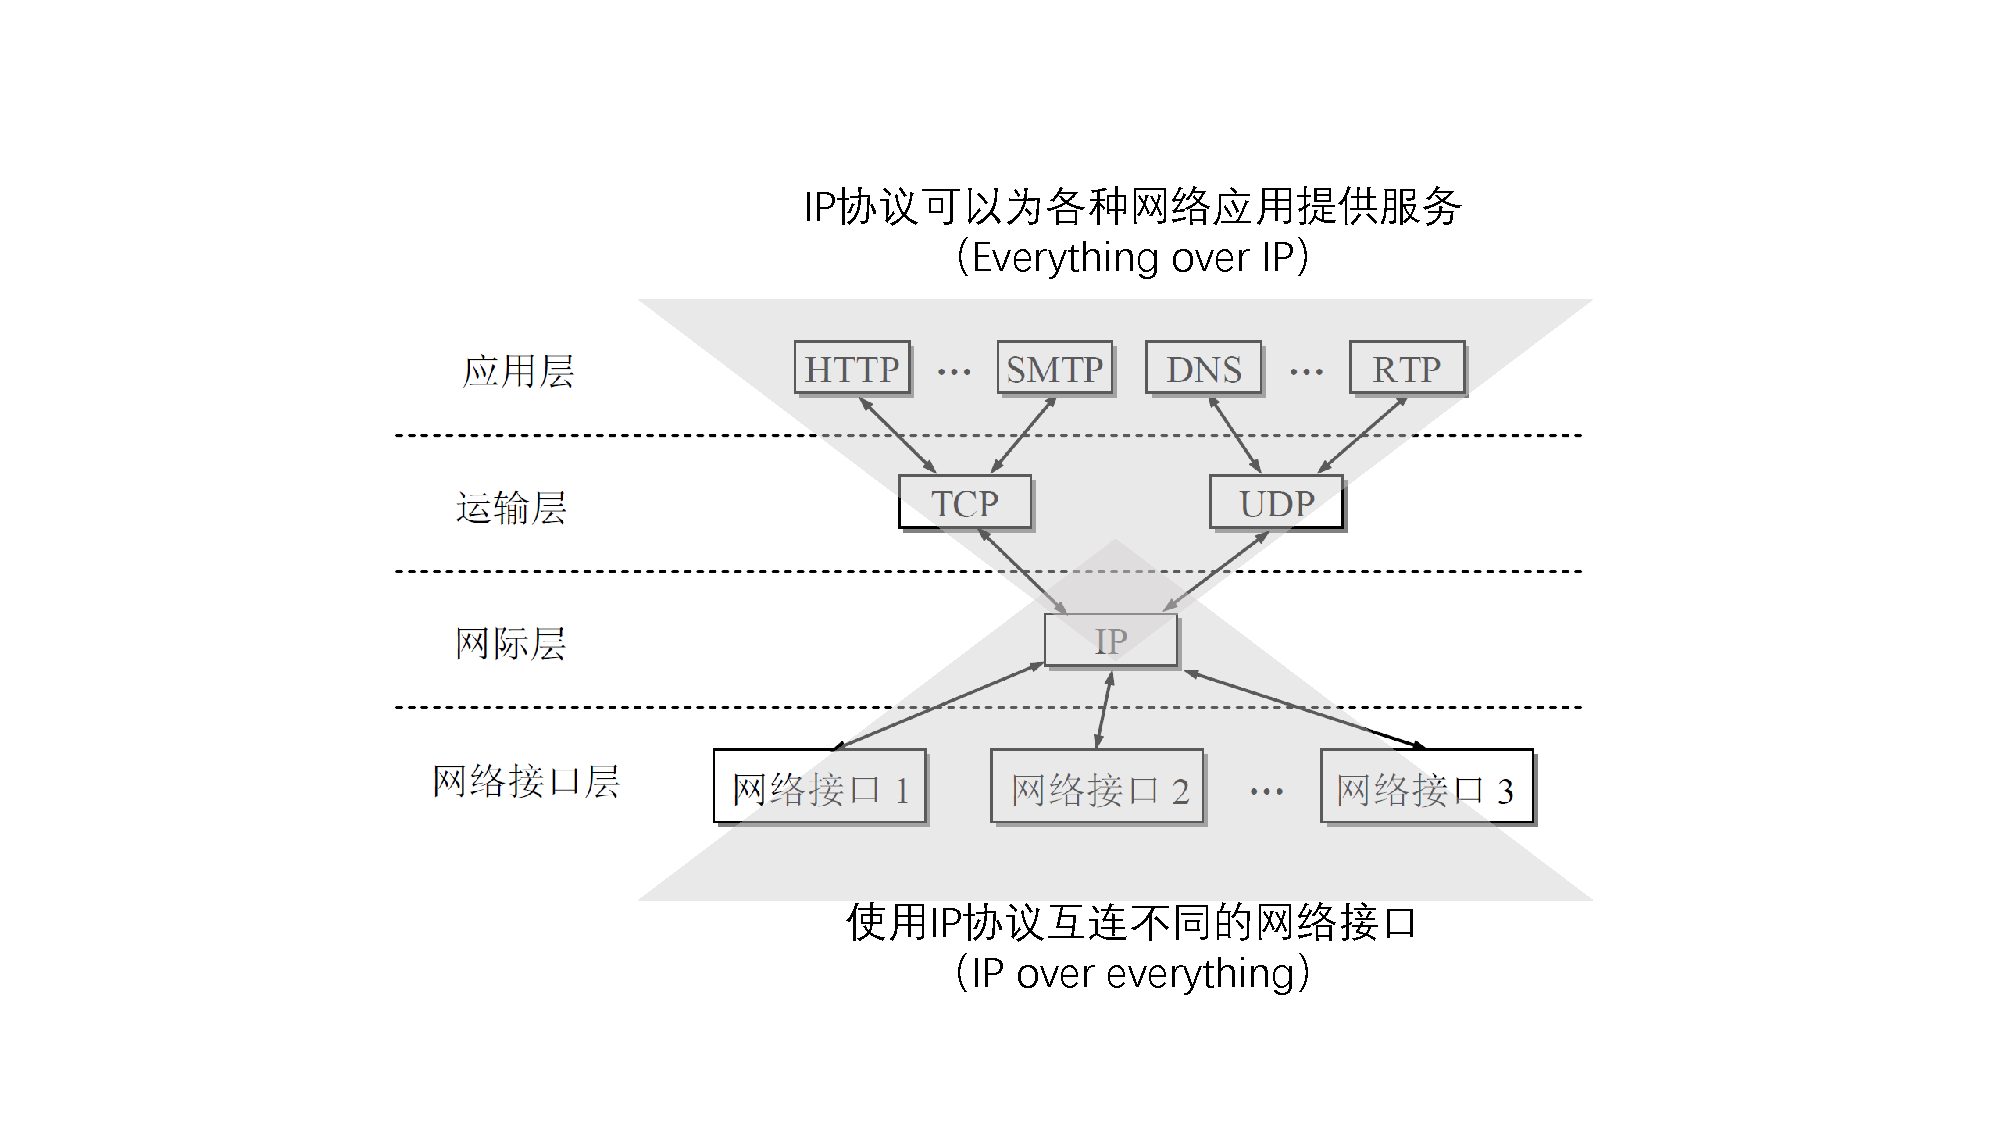
\includegraphics[width=0.65\textwidth]{img/1.24}
	\end{figure}

	\subsection{计算机网络体系结构中的专用术语}
	\begin{itemize}
		\item 实体:任何可发送或接收信息的硬件或软件进程
		\item 对等实体:收发双方相同层次中的实体
		\item 协议:控制两个对等实体进行逻辑通信的规则的集合
		\item 服务:在协议的控制下,两个对等实体间的逻辑通信使得本层能够向上一层提供服务
		\begin{itemize}
			\item 要实现本层协议,还需要使用下面一层所提供的服务
			\item 协议是“水平的”,服务是“垂直的”
			\item 实体看得见相邻下层所提供的服务,但井不知道实现该服务的具体协议。也就是说,下面的协议对上面的实体是透明的
		\end{itemize}
		\item 服务访问点:在同一系统中相邻两层的实体交换信息的逻辑接口,用千区分不同的服务类型
		\item 服务原语:上层使用下层所提供的服务必须通过与下层交换一些命令,这些命令称为服务原语
		\item 协议数据单元 PDU:对等层次之间传送的数据包称为该层的协议数据单元
		\item 服务数据单元 SDU:同一系统内,层与层之间交换的数据包称为服务数据单元
	\end{itemize}

	\begin{figure}[H]
		\centering
		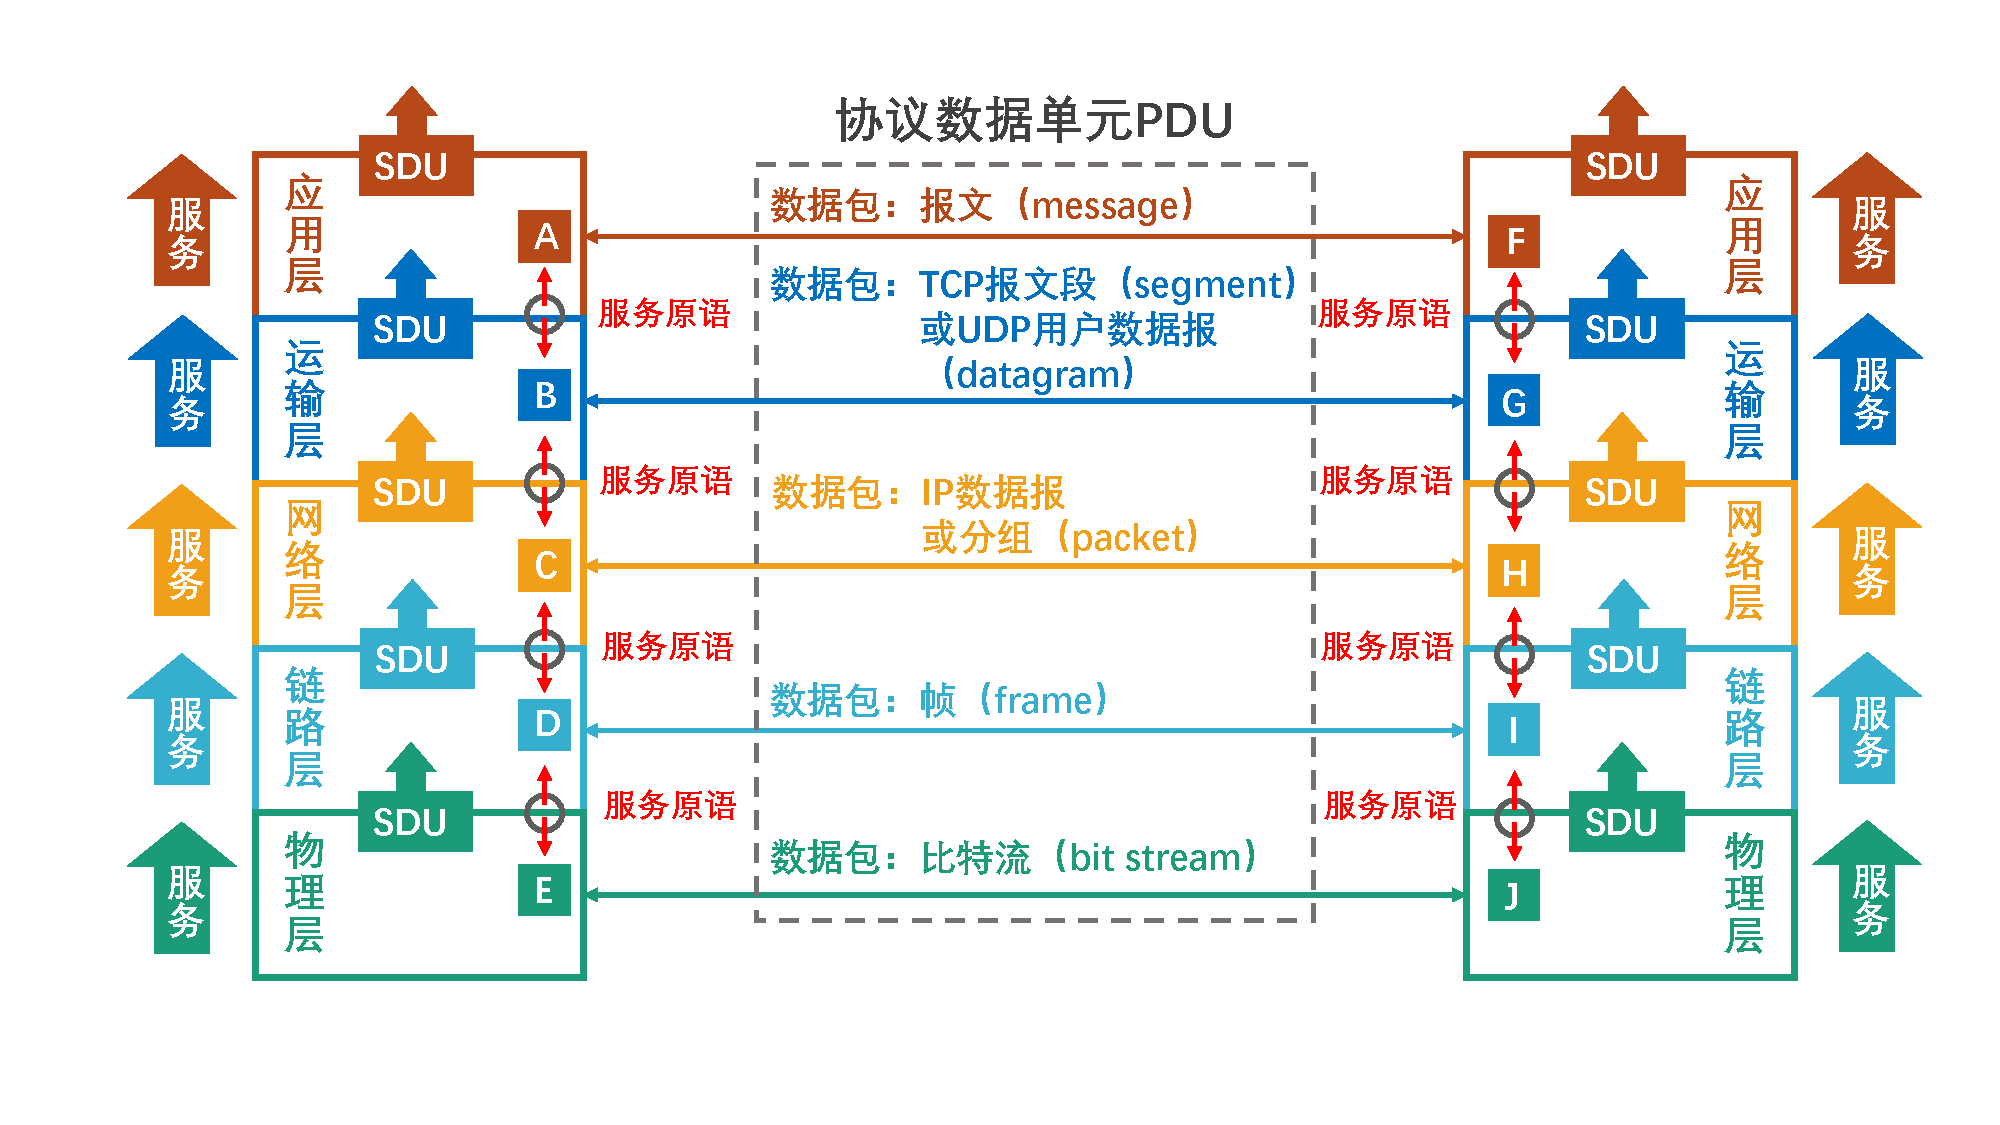
\includegraphics[width=0.95\textwidth]{img/1.6.4}
	\end{figure}

	
\end{document}


